\documentclass[a4paper,11pt]{report}
\usepackage{graphics}
\usepackage{color}
\usepackage{epsf}
\usepackage[pdftex]{graphicx}
\usepackage{subfigure}
\usepackage{setspace}
\usepackage{cite}
\usepackage{makeidx}
\usepackage{footmisc}
\usepackage{url}
\usepackage{multicol}
\usepackage[pdfborder=0 0 0]{hyperref}

\usepackage[T1]{fontenc}
\usepackage[sc]{mathpazo}
\renewcommand{\ttdefault}{cmtt}
% \linespread{1.05}         % Palatino needs more leading (space between lines)


\addtolength{\textwidth}{\oddsidemargin}
\addtolength{\textwidth}{\evensidemargin}
\addtolength{\textwidth}{-1cm}
\addtolength{\textheight}{1.5cm}
\setlength{\oddsidemargin}{0.5cm}
\setlength{\evensidemargin}{0.5cm}
\setlength{\topmargin}{0in}

\bibliographystyle{apalike2}
% TODO: \emph stuff
%TODO: Spanning Tree To Correct Language
\begin{document}

\begin{titlepage}
 
\end{titlepage}

\begin{abstract}
 
\end{abstract}

\tableofcontents

\chapter{Introduction}

Molecular Dynamics is an area of computer science and computational chemistry where computers are used to determine properties of materials and how collections of molecules interact with each other. Often these simulations are the only method that theoretical chemists have for investigation. Laboratory experiments cannot give sufficient detail in order to determine the microscopic properties of materials, but are good at determining the macroscopic properties of materials, for instance colour changes and temperature changes.

The most popular use for Molecular Dynamics is for Protein Folding, which is important for determining the structure of proteins. Protein folding is a process where a strand of amino acids(the protein) uncoil and form a 3D structure. The structure is determined by only the make up of the strand. Using this information, one can simulate an initial strand of amino acids and simulate it to determine what structure is formed. The use of distributed computing in Molecular Dynamics simulations, where multiple computers are used in the simulation, became popular with the release of Folding@Home.

The simulations that are run typically generate a lot of data. The simulations need to be run at a very small timescale, on the order of $10^{-12}$ seconds and can contain thousands of atoms. All of which needs to be saved in order to be studied by an expert user, a chemist or biologist, at a later date. Certain simulations, known as explicit solvent simulations, consist of a large amount of water molecules, or other solvent, surrounding an object of interest. In these simulations, there are usually many more atoms as each solvent atom needs to be represented.

For many simulations, compression is particular important as it can take an exceedingly large amount time to transmit all the data over slow internet connections. Our system will be specifically designed to tackle the problem of compression using the large amount of water molecules.

\section{Research Question}

Our research will attempt to establish which compression scheme is best for molecular simulations. We will determine which scheme is best by using two metrics for two criteria: compression rate and compression speed.

We will define the compression rate as the ratio between the original file size and the compressed file size. This yields a percentage where a lower number implies high compression was acheived and a higher number means a less effective compression. The speed of a compression will be defined as the number of seconds taken to perform the compression.

The key success factor will be if we can determine if a particular scheme performs best. Work from the project could be included in another project, so determining the best scheme is important.
 
\section{Implementation}

To determine these results, we implemented a system through which experiments could be done. The system is built-up of two sections: a compression section and a molecular visualisation section. The compression section contains all the compressors and the shared components required for each compressor to work. Each compressor is able to be run via separate drivers. The visualiser component is able to show the output of compression. Each compression scheme uses a process called quantisation where the atoms are irreversibly transformed to make compression more amenable. The visualiser facilitate the viewing of the transformation.

\section{Ethics}

There are several ethical issues that are relevant to our project. The first issue is with the quantisation process. Since the process is irreversible, the users must be aware that the compressed file does not necessarily represent the original simulation. The quantisation process, however, is a necessary part of compression. The user is also able to select the level of quantisation in order to balance the trade-off between simulation fidelity and compressed file size. 

We use several libraries in our system. On the compression side we use the Approximate Nearest Neighbours library(ANN) in order to determine information about the water in the simulation. We also use QT, a graphical user interface library, and GTS, a library for surface decimation, for the visualisation process. All of these libraries are released under LPGL, which allow us to use them in non-commerical products. As a result of this, the license that we have chosen for our project is the MIT license.

\section{Outline}

In Chapter 2 the background necessary for the project is discussed. This is followed by the design of our project in Chapter 3 and the implementation specifics in Chapter 4. Results and Analysis will be presented in Chapter 5. Finally, we conclude with a discussion of the main impact of our project and possible future work in Chapter 6.


\chapter{Background}

[TODO: fix labels]
There has been a great deal of work in compression over the past two decades[TODO: general compression reference], however, there is very little research on compressing Molecular Dynamics data specifically.
The following sections will describe the background necessary to an understanding of our approach.
Section \ref{back_mdf} describes the most dominant format that is used for storing the simulations on hard disk,
while sections \ref{back_intra} and \ref{back_inter} describe various techniques used in the related field of video compression.

\section{Molecular Dynamics Formats}
\label{back_mdf}

There are several Molecular Dynamics Simulation formats. Chief among these formats is the binary DCD file. This is the principle format used in Visual Molecular Dynamics(VMD)\cite{vmd}, a popular program for visualisation of molecules and simulation. This format also relies heavily on an existing PDB file in order to make sense of the output.

The PDB file stores information about each specific atom in the simulation. This generally includes the atom's element group, the latter is only important for use in protein simulations.[Possibly a reference here?] The data in the PDB file is stored in ASCII so the file is often larger than necessary. However, the PDB file only stores some initial information for each atom rather than for each frame in the simulation. The DCD format consists of the frames of the simulation containing all the atom's positions for each timestep. For this reason, a large amount of information is redundant when using DCD files in conjunction with PDB files: The PDB file stores positions for each atom, which are ignored when a DCD file is loaded. This means that the PDB files are much smaller than the corresponding DCD files and as succompressing the DCD files is the main priority for our project.  The main reason for the redundant information is to enable the molecules to be viewed in their normal state using just the PDB file and nothing else.

\subsection{DCD format}
The DCD format has various types which all differ slightly from each other. These differences may be ignored for most purposes, as they are normally stored as extra information in the header of the DCD file. VMD is able to handle all major variants such as the CHARMm and X-PLOR formats. However the most popular used is the X-PLOR format. \cite{vmddcdformat}

All these types have very slight differences which are mainly for keeping information about the original simulation, for instance the timestep between each frame. The DCD file format does not specify a prefered endian representation. The endianess of the data can be identified by magic numbers stored in the header, but any system that allows for loading DCD files must be able to handle both little and big endian correctly. The header also contains information relating to the number of atoms and the number of frames in the simulation.

The majority of the file is dedicated to storing the frames of the simulation. Each frame of the file represents a single timestep in the simulation. In each frame the positional information about each atom is stored. The positions are stored as triples of $x$, $y$ and $z$ 4-byte single precision floating point numbers. This makes up the majority of the file, as each atom repeated in every frame requires 12 bytes to fully specify. The order of the atoms in the frame is important as they correspond to the order of the atoms in the PDB file. No further information is stored in the file after the end of the final frame. The size of the final file can be estimated using the formula: 

\begin{center} $size = 12*frames*atoms$ bytes\end{center}

The above formula is only an estimate as it does not account for the header. Another problem is that in certain format types there can be atoms which remain fixed in space for the duration of simulation. These atoms are only stored in the first frame rather than in all frames. It is reasonable to ignore these effects in most simulations as they typically only account for a fraction of the original atoms. In all the simulations we looked at, none have any fixed atom information. [TODO: Incorporate John Stone email to next thing] Molecular simulations may have millions of atoms stored at each step and can involve many thousands of frames. This can result in files that are several gigabytes in size and in extreme cases, several terabytes in size.

These simulations need to be archived so that they can be reviewed by a molecular biologist at a later date or   they may need to be transmitted over relatively slow connections such as the Internet. Given their large size, it is often necessary to use compression.

\section{Molecular Simulation Compression}
\label{back_msc}
To date, there has been little research on compressing large-scale molecular dynamics simulations. The current method\cite{RefWorks:3} for compression is able to acheive output sizes smaller than the original by an order of magnitude. The method does not have any specific name, so for the remainder of this report we will refer to it as Omeltchenko's algorithm. There are two other algorithms of note that are useful for this situation. These are the Gandoin \& Devilliers Algorithm[TODO: cite] and the Predictive Point Cloud Compression Algorithm[TODO: cite]. Both of which are used for compressing point cloud data. A point cloud is a collection of points, where each point has position and possibly other attributes. This is of releavance because atoms stored in a PDB file may be treated as a point cloud.

\subsection{Omeltchenko's Algorithm}


The algorithm works by quantising the space that the simulation occurs in. This space is usually taken to be the axis-aligned bounding box that encompasses all the atoms, and this has to be recalculated on a per-frame basis. A three dimensional grid of a particular granularity is embedded into the space. Atoms are snapped to the centers of the closest grid cell. This transformation introduces a small error, which can be controlled by the granularity of the grid, but enables the algorithm to reduce the floating point coordinates to integer-based grid cell indices. This step, known as quantisation, is commonplace in point compression. It allows insignificant variations in the data to be removed, while introducing a quality setting to allow for better compression at the cost of accuracy. This stage produces a quantised $(x, y, z)$ coordinate for each atom. As a post operation, the points are translated so that all coordinates are non-negative. This process is made reversible by storing the bounding box of the original atoms.

The atoms' indices are mapped to Octree Indices. An Octree is a spatial partitioning data structure[TODO: ref], which recursively splits space up into 8 subdivisions. The subdividing process typically stops when there are few points in a cell or a maximum depth has been reached. A related variant of Octrees is Linear Octrees[TODO: ref], where the data structure is represented in a 1D array. Instead of using pointers in a tree data structure, the Linear Octree uses arithmetic in an array to calculate each node's index in an array. This usually uses more memory than a normal Octree as it requires the tree to be complete, however we are not interested in constructing the Linear Octree, only calculating the indices at which atoms would fall under. Octree Indexing is a reversable spatial hashing algorithm where 3D points are mapped to 1D indices, by using the Linear Octree cells. In this case, the quantised points are mapped to single non-negative integers. The algorithm uses Octree Indexing to interleave the bits of the coordinates of each point. The index, itself, is cleverly assembled so that points are only interleaved up to the largest most significant bit of every coordinate.

\begin{figure}
 \center
 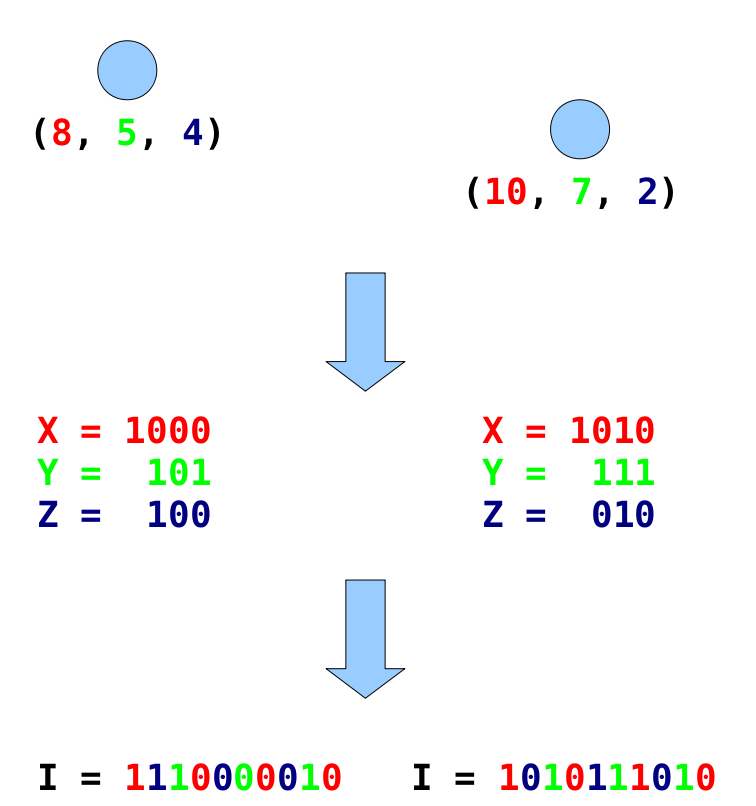
\includegraphics[width=0.5\textwidth]{resources/OctreeIndexingVerticalCropped.png}
\caption{Demonstration of the Octree Indexing Process on a system of 2 atoms. The first step of the process is conversion to binary. From this we can see that the $x$ components require 4-bits to encode as an index, while the $y$ and $z$ components require 3-bits. The final step of the prcoess is the interleaving of the bits in each atom's coordinates to produce a final number. }
\label{octree}
\end{figure}

The resulting indices are stored in a list and sorted in increasing order. These indices are written to the file using a delta encoding scheme. The first atom's position indicates its actual grid index, while the rest are stored as differences between the previous index and the current one. This final transformation typically allows a better compression rate to be acheived. Delta encoding reduces the amount of data that needs to be compressed by keeping things small and making it more amenable for compression, however it introduces a dependancy on decoding all the previous atoms in the list first. The output, itself, is performed by an adaptive, variable-length compressor. Typically, each index can be stored in a single 4-byte integer which results in an immediate size reduction from 12-bytes per atom to 4-bytes per atom. 

The compressor encodes the molecular data as a series of non-negative integers. Each integer streamed into the compressor one at a time. The compressor maintains an integer $l$ which is the current size at which integers are encoded as. As each integer comes in, it is checked to see if the integer can be stored using $l$ bits. If it can, it is stored as $l+1$ bits; a 0-bit followed by the bits of the integer. If it cannot, the integer is partly stored as $l+1$ bits; a 1-bit followed the first $l$ bits of the integer. The rest of the bits are compressed in the next step of the compressor. If enough of these overflows occur, $l$ is incremented.

The compressor was designed to be computationally undemanding as computers at the time of the paper were not as powerful as current machines. We found that it is not a good compression system as it is not based on any of the established variable-length encoders, which have been shown to produce near-optimal encodings.

The paper does not use the common file formats such as those used in VMD, it does, however, treat atoms very similarly so we are able to use the scheme for DCD file compression. The algorithm deals with atoms that are represented by a block of 56-bytes, containing position (24-bytes), velocity (24-bytes) and an ID (8-bytes). The paper claims that the 56-byte atomic data is encoded at approximately 6.3 bytes per atom. In our application, however, the atoms are defined only as 12-byte position data, but have an implicit ordering from the PDB file. Since the sorting destroys the ordering, additional information will need to stored to recover the initial ordering when decompressing.

\subsection{Gandoin \& Devillier's Algorithm}

[TODO: Diagram]
The Gandoin \& Devillier's Compression Algorithm exploits a property of KD trees[TODO: cite] to compress Point Cloud Data.\cite{devillers2000gci} A KD tree is a spatial subdivision data structure which partition space using various axis-aligned splitting planes. The KD tree cycles through each dimension for the splitting axis as the data structure is recursively constructed. The splitting planes are chosen to divide the space in half at each step. This differs from Octrees in they space is divided. Octrees split space into four subdivisions of equal area, while KD trees only split space into two and do not require that the areas are equal.

Gandoin and Devillier's algorithm exploits the property that if one knows the number of points over the entire space and the number of points in one of the regions created from the split, one can work out the number of points for the other region by arithmetic.

Each leaf node of the tree is subdivided if there are multiple points in the region. The points in the compression are usually quantised. The original frame may only have distinct points, however, the quantised frame could have several duplicates depending on the quality of the quantisation. For this reason, the subdivision might stop before the number of points in a cell is less than 2.

An advantage of this algorithm is that it is progressive. This means that low-detail representations of the point cloud can be constructed from the initial parts of the compressed stream. As the compression progresses the detail in the model becomes finer until the output reaches the final quantised result. This algorithm produces a symbol stream which is usually encoded with an entropy encoder such as Arithmetic Coding.[TODO: cite]

\subsection{Predictive Point Cloud Compression Algorithm}

[TODO: diagram]
Predictive Point Cloud Cloud Compression is a new approach to compressing point cloud data. The compression scheme creates a spanning tree of the original point set using heursitics.\cite{gumholdcomp} Predictors based on these heuristics exploit patterns in the data to get an estimate of the position of a child in the tree relative to its parent. The use of these predictors means that only the residual error from each prediction needs to be stored.

In the original paper the algorithm only used one of two predictors for the entire models to encode the entire pointset. The user was prompted for which predictor to use. The first predictor predicta that the child would be placed in the same position as the parent, while the second predictor estimates the child to have the same displacement as the displacement between its grandparent and parent. Further enhancements to the algorithm were made to choose the best predictor at each step of the algorithm and also extra predictors were added.\cite{merrycomp}

The performance of this algorithm depends greatly on the quality of the predictors used. Poor predictors will result in significantly worse compression. The compression scheme requires the number of small errors to be high, and decays very rapidly as the the error size increases. The predictors also require that the point cloud represent a surface so that information such as the surface normal at each point can be estimated.

\section{Video Compression}

A different approach to follow is that of video compression. Essentially, the molecular simulations can be viewed as videos, but using 3D molecular data instead of 2D picture data. We can safely ignore the audio part of compression as it bears no relevance to molecular simulations. Video Compression loosely falls into one of two subcategories. The first is intraframe compression which seeks to compress each individual frame using little or no information about previous frames. The other type is interframe prediction which uses a significant amount of information from previous frames to compress a frame. 

Usually, each frame is heavily analysed for objects that are considered important. These objects are often major features such as a person's arm or a ball. The purpose of the intraframe compression is to record these objects with their initial positions, while interframe prediction estimates the position of the objects and only records the errors that occur from making the estimate. In most cases, given a good predictor, the error is usually small and can be compressed very well.

The rest of this section will discuss the algorithms used in both intraframe compression and interframe prediction. The techniques used to detect objects in the images are ignored, as our simulations have atoms which are already defined objects.

\subsection{Intraframe Compression}
\label{back_intra}

The latest MPEG encoding algorithms allow for a choice of several compression algorithms to be used\cite{gall1991mvc}. This section will focus on the most common algorithms used for compressing the objects in the original image. These algorithms can be classified as either lossless or lossy. Lossless compression algorithms are able to recreate the original data with no loss of information. These lossless compression algorithms are general enough to apply to standard data compression. Lossy compression algorithms, on the other hand, are able to achieve much higher compression rates, but do incur the penalty of some information loss. Typically, the lossy compression algorithms first quantise the input to fit within a certain number of symbols and still require further compression from a lossless algorithm. We will focus mainly on the lossless compression techniques as information loss, aside from small quantisation errors, may result in incorrect assumptions being drawn from simulations.  

These techniques fall into two categories: Entropy encoders and dictionary encoders. 

\subsubsection{Entropy Encoders}

Entropy encoding makes use of Information Theory and tries to build an optimal mapping from symbols in the frame to individual bits. In a video frame, this information could be lossily compressed blocks of pixel data or information about identified object. In a molecular simulation we could easily use this to store positions of molecular data.

The first algorithm of this type developed was Huffman Encoding\cite{citeulike:1320251}. The original Huffman Encoding relies on having frequencies of all symbols that occur in the message. It uses this table to build up a prefix-free tree. A prefix-free tree's leaves are symbols and the paths from the root to a leaf indicates the bits required to output that symbol. The frequencies allow the algorithm to construct an `optimal` tree that requires less bits to output common symbols and more bits to output rare symbols. Decoding a single symbol from a message  entails following the paths indicated by the bits until a symbol is reached, or looking up the bit patterns in a table or codebook.

\begin{figure}
 \center
 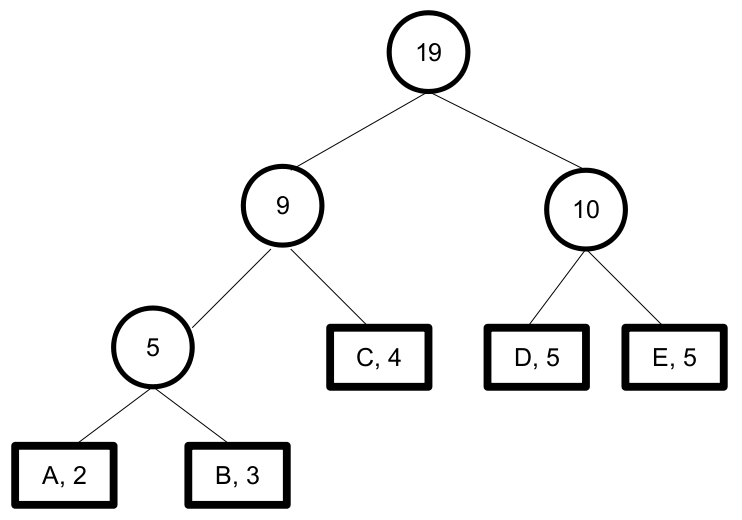
\includegraphics[width=0.4\textwidth]{resources/HuffmanTreeCropped.png}
\caption{A Huffman Tree for a simple alphabet of \{A,B,C,D,E\} with frequencies \{2, 3, 4, 5, 5\}. A and B have a comparatively low frequency to the C, D and E and thus require more bits to encode. The codebook constructed from this tree would be \{A: 000, B: 001, C: 01, D: 10, E: 11 \}}
\label{huffman}
\end{figure}

There are various issues when using regular Huffman Encoding. The first problem is that the entire message must be available when writing the compressed data in order to compute the frequency table.\cite{RefWorks:1} The second problem is that in order to decompress we need to also output the entire prefix-tree used for compression. These problems can be remedied by Adaptive Huffman Encoding\cite{42227} which is able to re-optimise the prefix-tree while the compression occurs.

The Adaptive Huffman Encoding scheme is a good candidate for compression of the molecular simulation frames. The memory footprint of the algorithm is low: only the prefix-free tree needs to be stored while the algorithm runs and has a worst-case space usage of $O(S)$, where $S$ is the number of unique symbols in the frame. The algorithm can also be run while the simulation takes place as only a small amount of computation needs to occur per atom.

There is a similar entropy-based compression algorithm called Arithmetic Coding. This algorithm has an advantage over Huffman Encoding as it can store symbols as a fractional number of bits. \cite{RefWorks:1}, \cite{RefWorks:3}. The amount of wasted bits that appear in Huffman Encoding can be as bad as 1 bit per symbol. Arithmetic Coding works by encoding the entire message into a single rational number in the range [0, 1). The frequency of each symbol is used to allocate large subranges to frequent symbols and small subranges to rare symbols. 

\begin{figure}
 \center
 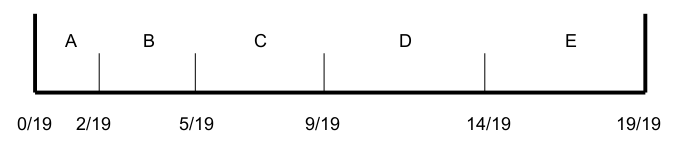
\includegraphics[width=0.8\textwidth]{resources/ArithmeticCoder.png}
\caption{Arithmetic Coder ranges for same alphabet in Figure \ref{huffman}}
\label{arithmeticcoder}
\end{figure}

Encoding a specific symbol simply requires adjusting upper and lower bounds of the output number. When the entire message is encoded the number can be output. Decoding requires one to follow the subranges that the encoded message falls into.

\begin{figure}[h]
 \center
 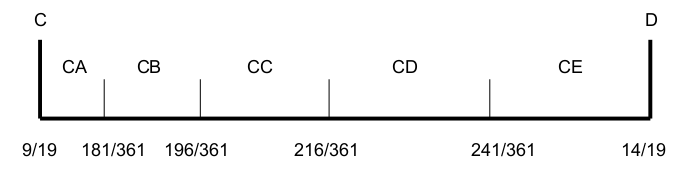
\includegraphics[width=0.8\textwidth]{resources/ArithmeticCoderSubrange.png}
\caption{Arithmetic Coder ranges after encoding a C}
\label{arithmeticcodersubrange}
\end{figure}

[TODO: image wrong]

Arithmetic Coding implementations are typically very complex. Some implementations use a static dictionary of 256 symbols, while others are able to handle a dynamic dictionary of up to a few thousand symbols. The reason for this is that the numbers for the ranges are not implemented using an arbitrary precision rational number library. Instead they use a representation based on regular 32-bit integers. Overflow and underflow issues are handled by scaling the range.

Unfortunately, there are problems with the original arithmetic coding algorithm in that you need to compute the entire frequency table so that it can be output before compression begins. The Adaptive Arithmetic Coding algorithm is an adjustment that does not require the frequency table to be constructed beforehand, but it does, however, require that symbols are stored prior to any output. 

Both the Adaptive Arithmetic Coding algorithm and the Huffman Coding algorithm require a separate component for handling the frequency table. Unlike, the regular static algorithms, this frequency table needs to allow insertion of new symbols, updating the frequencies of existing symbols as well as determining which symbol a given frequency belongs to and what the frequency range of a symbol is. Two common data structures for storing this information are arrays and Fenwick Trees.[TODO: reference]
%The two most common data structures for this are range trees[TODO: cite] and Fenwick trees[TODO: cite].

In most implementations of Arithmetic Coding, the encoding algorithm is separated from the static or adaptive parts of the algorithm. The core algorithm is usually called the encoder and decoder, as it is only responsible for encoding and decoding ranges. The encoding and decoding part is independant of whether one uses the adaptive or static algorithm. The parts of the algorithm that handle the adaptive and static part is called the model. This separation allows for better modularity and design of an arithmetic coder.

The Arithmetic Encoding scheme offers a better choice for compression of the frames. The adaptive models allow us to update symbol frequencies while the frame is being compressed. This leads to the same worst-case space usage as Huffman Encoding. The adaptive algorithm also requires only a small amount of computation per symbol. However, the problem of conveniently storing the symbols for each output file remains.

\subsubsection{Dictionary Encoders}

Dictionary-based encoding schemes attempt to compress data using a different approach from entropy encoders\cite{RefWorks:2}. A data structure known as a dictionary is able to efficiently keep track of a sliding window of text information. This window allows different dictionary encoding algorithms to take advantage of distributions of symbol placement data in the input message. Rather than using frequencies as a basis for shorter codewords, they resort to greedily assigning symbols or groups of symbols to codewords of increasing length. This gives certain advantages over entropy encoders, such as speed and requiring little or no mapping information necessary to decode the data. 

There are various dictionary-based compression algorithms, key among them are the LZW and DEFLATE algorithms. The Lempel-Ziv-Welch(LZW) algorithm keeps an explicit dictionary that is progressively built up as the stream is read.\cite{1320134} Using this information, a codeword for the current symbol can be worked out and written to file. This algorithm needs to store additional information with the text in order to reconsitute the initial dictionary, but after this the message can be recreated by dynamically updating the dictionary. 

The DEFLATE algorithm uses several techniques such as an additional layer of Huffman Coding for bit-reduction, a sliding window based dictionary and a duplicate string removal algorithm\cite{deflaterfc}. It is the most commonly used dictionary-based compression algorithm and is used in applications such as gzip and in the PNG image format. 

Dictionary-based encoding schemes tend to perform worse on average than entropy-based encoders, but can perform much better for certain messages, for instance, where there are large runs of repeated information. Dictionary-based encoding schemes require very little computation per symbol and have low memory overheads. However, these overheads can be larger than in entropy encoders. 

% \subsubsection*{Vector Quantisation}
% 
% Vector Quantisation is a common technique used in video and speech compression systems.\cite{RefWorks:1} The mechanisms, by themselves, do not compress the algorithm, but instead attempt to reduce the number of unique symbols that are used in the frame. This output is then used as input for a lossless compression scheme such as Huffman Encoding. Vector Quantisation algorithms acheive this symbol-reduction by considering the symbols to exist in some N-dimensional vector space. This space is then split up into various cells whose identifiers will be used as the symbols to compress. The mapping from symbols to cells must also be stored in the compressed output.
% 
% The first algorithm for creating the cells is known as Lloyd-Max algorithm.\cite{108235} The iterative algorithm creates a Centroidal Voronoi Diagram. A Centroidal Voronoi Diagram is a subdivision of N-dimensional space into $L$ cells. Each cell has exactly one point assigned to it, which is the centroid of each cell, and the cell is defined as the volume of space which is closest to the cell's point. The centroidal property keeps the information lost in the transformation at a minimum.\cite{RefWorks:1} The algorithm's complexity increases exponentially as the dimension of the space increases which makes it infeasible in even low dimensions.\cite{116880}
% 
% The second algorithm for creating the cells is the K-means algorithm.\cite{1979} This is an iterative algorithm which differs from the Lloyd-Max algorithm by using the mean of the cells instead of the centroid. This adjustment negates the need for a Voronoi Diagram and thus it often outperforms the Lloyd-Max algorithm, however the quality of the cells generated is a trade off.
% 
% These algorithms are only slightly applicable to the domain of molecular compression. The first trade off that we have made is the loss of information in the simulation. This is countered, however, by being able to acheive a much higher compression rate than lossless encoders. They also need an entire frame of information in order to run and thus lead to a higher memory usage. They can also be infeasible to perform alongside a molecular dynamics simulation.
% 
% \subsubsection*{Transform Coding}
% 
% Transform coding is another group of image compression algorithms which attempt to reduce the detail present in a frame. They are suited towards images due to the large amount of numerical information that allows the transformation to occur. These transformations are typically followed by a lossless encoding scheme.
% 
% The first such transform was the Discrete Fourier Transform\cite{Cody92thefast}. This algorithm transforms the digital signals, the pixels, into analogue signals which represent the image. These signals can be analysed using a frequency analysis. The signals have different effects on the image. Lower frequencies determine the large scale structure of the image, while higher frequencies are responsible for detailed parts of the image. A function called a convolution, in this case a low-pass filter is applied to cut off any high frequencies, reducing the detail in the image.\cite{1464352} The Discrete Fourier Transform was later replaced with the Discrete Cosine Transformation, as Discrete Fourier Transformations tend to perform worse around the borders of the image\cite{RefWorks:1}.
% 
% Transform coding is a commonly used lossy compression scheme in image and video compression. However, the same problems as with Vector Quantisation occur. It requires an entire frame to be streamed in before any compression can begin. It will also perform poorly in molecular simulations because we are compressing a atom point list instead of a volume of space. They also require slightly more computation than regular lossless encoding schemes.

\section{Interframe Prediction} 
\label{back_inter}

Interframe prediction takes advantage of the correlation between the current frame and previous frames. Objects that are identified are predicted to be in a new position. Most of the time, the prediction will be incorrect, but, if the predictors are chosen carefully, the predicted position will be close to the actual position. If the errors are small, they can be effectively compressed, using an entropy encoder, as individual errors are likely to occur more frequently. There are several types of prediction that in common use. We will discuss, specifically, first-order prediction, K-th order prediction and Kalman Filtering.

There are several noticable differences with the prediction schemes suitable for standard video formats and the molecular dynamics simulations. The first difference derives from the fact that these schemes require some information to bootstrap the prediction. Frames in molecular dynamics simulations can use positions of the atoms in previous frames to predict on, while videos often only have pixels. The latest compression schemes break the video up into blocks. Objects are identified within these blocks. Prediction can the be performed on the objects giving a high rate of compression. The MPEG-4 format specifies a single prediction scheme with a large number of features\cite{wiegand2003oha}. 

A related topic is that of index frames. One of the reasons this prediction is not used completely throughout a video file is that it makes every frame in the file dependant on all the frames that precede it. In order to decode a frame in the file, every prior frame must be decoded. To allow for random access in a video, certain frames are labelled as Index frames or I-frames which are compressed only using Intraframe compression. Typically, a structure called a Group Of Pictures will be given that defines the order of the I-frames, and predicted frames, or P-frames\cite{vandalore2001sal}. There are also frames that can predicted from the previous or the following frames, called B-frames. This structure is useful to have in any compression of molecular dynamics simulations since it allows for random access in the simulation using both intraframe and interframe compression.

\subsubsection{First Order Predictors}

First order predictors use the current velocity of an object as a predictor of where the object will appear in the next frame. The velocity is calculated as the difference between the positions of the object in the previous two frames. This scheme would be particularly easy to implement in a molecular dynamics simulation where objects are explicitly provided.

The error is coded as the difference between the predicted and actual position of the object. Given the physical nature of the simulations, this error is likely to be small, however, in a normal video there can be situations where this predictor does not perform very well.

[TODO: picture fix]
\begin{figure}[h]
 \center
 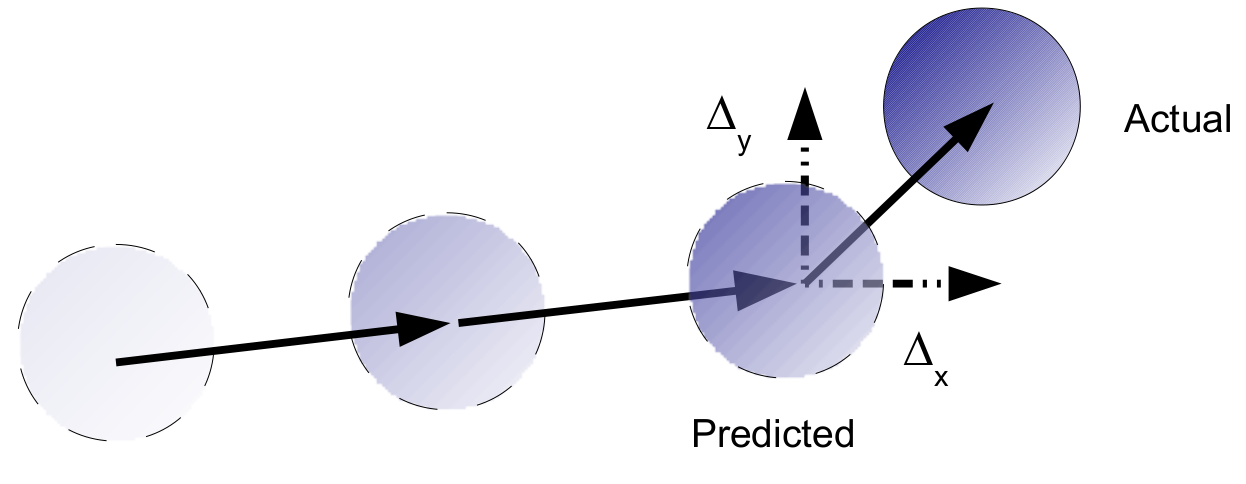
\includegraphics[width=0.6\textwidth]{resources/FirstOrderEncoding.png}
\caption{First Order Encoding of a point}
\label{linearencoding}
\end{figure}

\subsubsection{K-th Order Predictors}

K-th order predictors are an enhancement of the first order predictor. Instead of just the positional data of the last two frames, they use an object's positional data over the last $K+1$ frames to calculate the first $K$ derivatives of the object's position. Essentially, a curve is calculated that passes through all $K+1$ previous positions. These predictors are updated when the next frame is encoded and used to predict the next position of the object.

[TODO: picture fix]
\begin{figure}[h]
 \center
 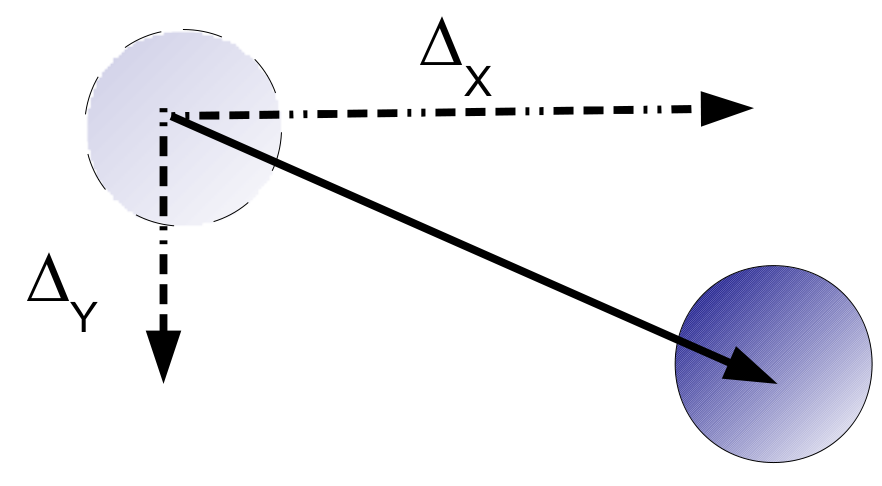
\includegraphics[width=0.6\textwidth]{resources/DeltaEncoding.png}
\caption{0-th order Encoding of a point, also known as delta encoding}
\label{deltaencoding}
\end{figure}

The error is again coded as the difference between the predicted and actual position of the object. However, there are several drawbacks to using K-th order predictors. The positional data of each of the objects must be kept from the previous $K+1$ frames. Also, each prediction requires $O(K^2)$ work to be performed per object. Another problem is that as $K$ increases, the quality of the predictions does not necessarily increase, and could even decrease, resulting in large error rates. If the points are not moving in a coherent fashion, that is their motion is not unpredictable, then this prediction will not do well.

\subsubsection{Kalman Filtering}

Kalman Filters are a relatively advanced prediction system that represent the motion of an object as a stochastic process.\cite{welch1995ikf} The predicted position at timestep $k$, $p_k$, of the object can be simulated as a linear stochastic difference equation of the form:
\begin{center} $p_k = Ap_{k-1} + Bu_{k-1} + w_{k-1}$  \end{center}
The actual measurement data, $x$, is related to the current predicted state by:
\begin{center} $x_k = Hp_k + v_k$ \end{center}
$w_k$ and $v_k$ are random variables which are normally distributed and are related to the noise that occurs within the stochastic process. $A$ is a matrix relating the previous prediction to the current prediction. $B$ is a matrix capturing optional control input, for instance additional prediction information. $H$ is a time-dependant matrix which relates the current prediction to the current actual measurement. The Kalman Filtering process adjusts the matrices within the equations to get better and better approximations of the motion of the object.

Kalman filters provides increasingly better predictions as more frames are encoded. The drawback is that several matrix multiplications are required to acheive this accuracy, which can be computationally expensive to do on a per-object basis. This is especially true in large scale molecular dynamics simulations where there could be millions of atoms. This extra computation, however, could have a dramatic impact on the rate of interframe compression due to the very small error rates.

\section{Summary}

There are two main techniques for compressing videos. Intraframe techniques reduce each frame to a collection objects, in molecular simulations these are the atoms, which are encoded using either entropy encoders or dictionary encoders. Entropy encoders include the techniques of Huffman Coding and Arithmetic Coding. Huffman Coding uses an algorithm to construct a prefix-free tree to map symbols to bits, but can waste up to $1$ bit per symbol. Arithmetic Coding is a more complicated technique which uses rational numbers to encode symbols. Arithmetic Coding can encode symbols as a fractional number of bits, avoiding the wastage that exists in Huffman Coding.

Interframe techniques use temporal coherence to better encode each frame, however this introduces a dependence on some of the previous frames. Interframe compression attempt to guess the next state of objects and encode any errors. If the predictions are accurate, a better compression rate can be acheived. There were two main techniques that were investigated. First order and K-th order prediction compute curves that fit data over a selected window of framesand extrapolate from this curve. Kalman filters treat the motion as a stochastical process that can be estimated with some accuracy through the use of matrices.

\chapter{Design}

[TODO: detail]

The project's main aim was to investigate how effective certain methods of compression would be on molecular simulations. Our system was thus designed in order to test the effectiveness of the compression schemes. Using our system we measure the performance of the compression methods, in terms of speed and size of the compressed file. The actual testing of the system is accomplished via scripting and not directly through our system.

\section{Design Methodology}

We settled for an iterative design methodology. The system was designed so that the first iteration would have very little functionality, but still be able to compress simulations. In the first iteration, only two compressors based on reference schemes were implemented. The second iteration had more compressors, including schemes based on interframe prediction. The third and final iteration had all the compressors and visualisation completed.

The initial design of the program consisted of an integrated system that could handle compression, decompression and visualisation of the molecular simulation data. This was changed once we learnt that the compression would possibly be included in VMD. VMD allows the simulations to be visualised using several different representations and so our visualisation would not be useful for VMD.

The program was then split-up into components that could be shared across multiple programs, namely the visualisation and the compressors. This was necessary as there was functionality that needed to be in both the visualisations and each compressor, such as quantising and dequantising points. The graphical front-end of the program would be handled entirely by Min-Young Wu, while the compression back-end would be split-up fairly between Keegan Smith and Julian Kenwood. 

Another motivation for splitting up the work load is that testing requires each part to be separated in order to more efficiently gather results. The final design allowed the compressors to run independently with a separate driver program for each one.

Another important design choice was to separate the Interframe and the Intraframe compression schemes. In normal video compression schemes they are combined into a single scheme. In order to adequetely measure the performance of the interframe compression schemes it is necessary decouple them. The use of other schemes would make it difficult to measure the compression time and compression rate. 
 
The system is designed to be very memory efficient. As little memory would be used as possible in order to carry out the compression. Our main reason for this was that the data we were dealing with was very large. Individual frames were potentially several gigabytes in size. The current state of the art in simulations has a much lower size limit of several megabytes.[TODO: John Stone Ref] The system that is implemented is less stringent on memory which simplifies it greatly.

The final requirements for the compression section of our system are that it would needs to be able compress large simulations with large numbers of atoms and frames. We define large simulations as consisting of at least:

\begin{itemize}
 \item $2,000,000$ atoms
 \item $10,000$ frames
\end{itemize}

From these requirements, we calculated that the size of each frame is about $20MB$ at maximum. The intraframe compression schemes only hold each frame once as they are being compressed. However, the interframe compression schemes require a window of previous frames. Typically, this window is very small, so the impact of storing each frame in the window is negligble.

It is predicted that in the next 2 years, the state of the art clusters will be to create simulations containing between $10,000,000$ and $100,000,000$ atoms. In order to handle these increases our system may need to be optimised in order to allocate as little memory as possible.


\section{System Overview}

\begin{figure}[h]
 \center
 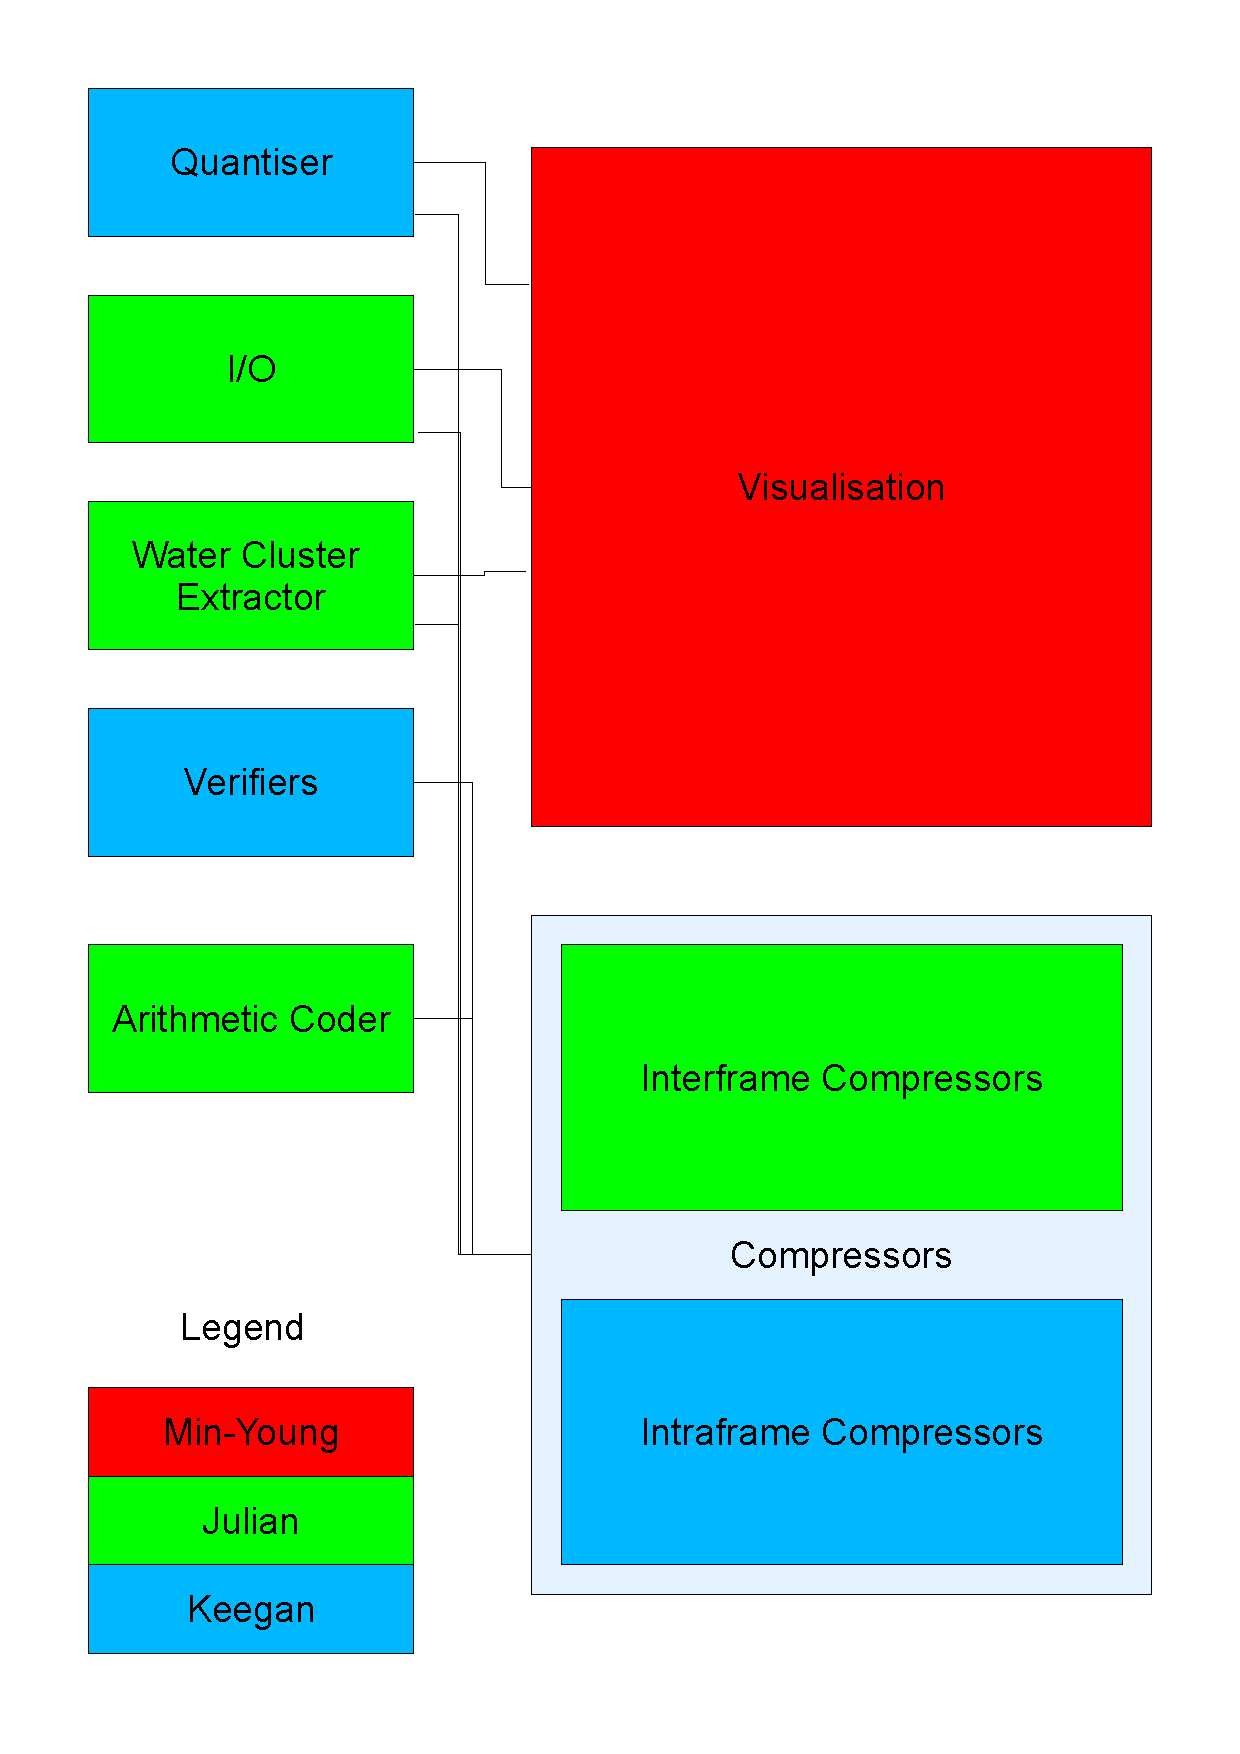
\includegraphics[width=0.5\textwidth]{resources/Breakdown-connect.pdf}
\caption{System breakdown}
\label{sysbreak}
\end{figure}

[TODO: reference all figures, add more section references]

The system is divided up into several sections(Figure \ref{sysbreak}): Visualisation, Compressors and Components. The Visualisation handles viewing of the output of molecular simulations that have been compressed by our system. It allows users to see the effects of quantisation on the simulations. This section was implemented by Min-Young Wu and is explained more thoroughly in his report. 

The Compressors section contains all the compression techniques that were implemented. The compressors fall into one of two subsections: Intraframe and Interframe compression. The Intraframe compressors were mainly implemented by Keegan Smith, although the Omeltchenko Encoder was implemented by Julian Kenwood and its implementation will be explained later in this thesis. (Section \ref{imp_omelt})

The Components part of the system represented various subsystems that are shared among various parts of the project. The main reason for separating these components out was to avoid code duplication. There are additional benefits such as easier testing and better subdivision of the work load among our team.

The following is a list of the components and their roles in the systems. \\ \\ \\

[TODO: beef up the next stuff]
\begin{itemize}
 \item Quantiser
 \begin{itemize}
   \item This component is responsible for the quantisation and dequantisation of the points in each frame of a simulation.
 \end{itemize}
 \item I/O
 \begin{itemize}
   \item These components performs I/O to and from the original DCD and PDB formats. 
 \end{itemize}
 \item Water Cluster Extractor
 \begin{itemize}
   \item The Water Cluster Extractor transforms the list of atoms into a list of water clusters and other atoms.
 \end{itemize}
 \item Verifiers
 \begin{itemize}
   \item These components verify the results of compression and gather statistics on the error in quantisation.
 \end{itemize}
 \item Encoder
 \begin{itemize}
   \item These components transform a list of symbols into a compressed bitstream.
 \end{itemize}
\end{itemize}


% This section will describe the design of the compression side of the project. The design of the visualisation aspect of the project is not described in this section as they are not necessary for measuring compression rates. The visualisation does, however, impact on some of the design choices required for the compression which are described in the appropriate sections.
% 
% To facilitate a well designed project, the compression aspect was split up into various components. These components act as transformations on input data, such as atoms in a frame, to produce required output data, for instance quantised atoms.

% These components are categorised in to several groups which relate to specific tasks that need to be accomplished. These groups are:



% Each of the components will be discussed briefly in the following section. Finally, there will be a discussion on the design of the experiments for recording the success of this method.

\section{Compressed File Format}

We chose a standard file format for all compressors. This decision simplified the implementation of the compressors and allowed easy addition of new compressors. The format has several sections that allow it to reconstitute an uncompressed DCD file.

The header of the file is broken up into two segments. The first segment stores the DCD file's header which includes the number of atoms and frames in the simulation. The second segment stores header information relevant to the compression. In many of the compression schemes this is only the quantisation levels, however some of the interframe schemes require additional information about prediction window sizes.

The remainder of the file consists of records, one per frame. Each record contains a frame header followed by the compressed data. The frame header contains information about the bounding box of each frame. Using the bounding box and the quantisation levels, a quantised approximation to the original data can be constructed. The compressed data section is specific to each compression scheme.

\begin{figure}
 \center
 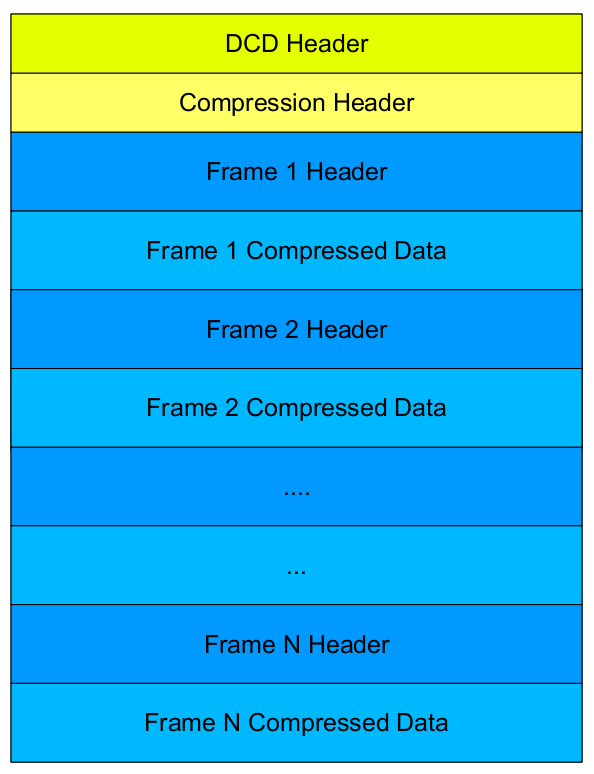
\includegraphics[width=0.4\textwidth]{resources/FileFormat.png}
\caption{Compressed File format: The green blocks represent per-file header information that is stored only once. The blue blocks represent data that occur in a per frame basis.}
\label{fileformat}
\end{figure}

% \subsection{Overview}

[TODO: Future implementation]

\section{Experiment Design}

The experiments that are performed for evaluating the system are designed to test both compression rate and speed of the implementations. The important questions that we are requiring to ask is which compressor performs the best. [TODO: this is not really the question I set myself to answer in the proposal, I believe I only had to answer the question for Omeltchenko and Predictive Pointcloud Compression while Keegan Smith handled the Gandoin \& Devillier's and Predictive Pointcloud Compression]

The performance of the schemes will be compared by measuring the compression rate and speed on two levels. For each dataset the compression rate and computation time will be measured for each simulation in the entire dataset. Using this data, a mean running time per atom can be determined as well as the variation of these running times. Significant running times ocan point to issues that can cause the algorithms to perform slower. A similar argument can be made for the compression rate. The causes of high variation may be determined by looking at the number of water clusters in each frame in the case of Predictive Pointcloud Compression, while Omeltchenko may require further information to analyse.

Several datasets will be used. The sizes of the simulations will vary from very large, approximately one million atoms with one hundred to one thousand frames, to very small simulations of only a few thousand atoms and a few dozen frames, with several datasets in between. There will also be datasets that consist completely and of water and datasets that contain no water. Finally, we will also have datasets that contain a very complex molecule in solution.

\chapter{Implementation}

This chapter will describe the implementation of each component used in the system.

\section{Intraframe Compressors}

Only one Intraframe Compression scheme was implemented by myself, the others were implemented by Keegan Smith. Implementation details may be found in his report. The reference Omeltchenko compression scheme is based on the algorithm outlined in [TODO: label to background chapter]

\subsection{Omeltchenko Scheme}

\label{imp_omelt}
The Omeltchenko Scheme was implemented with slight differences to the algorithm described in the paper. The algorithm was initially implemented with the prescribed sorting algorithm for sorting the list of octree indices. 

The paper describes using a large array of lists such that, for uniform distributions of atoms, maps approximately $O(1)$ atoms to each list. Each of the lists are then sorted using a heapsort and the merged into a final sorted list. The size of the array is equal to the number of atoms in the frame and divides the range of octree indices into roughly equal parts. The benefit of this approach is that, for uniform distributions, all indices can be sorted in approximately linear time.  In large simulations, the memory usage and overhead of running many heapsorts grows quickly. In order to reduce the running time, the paper suggests splitting the molecular simulation up into smaller boxes and then merging the sorted indices of these boxes. The paper does not give any instruction on how to split the simulation up. In our implementation, the STL sort is used. This is an implementation of the Introsort algorithm which has linearithmic worst case behaviour and is heavily optimised.

The encoding of each symbol in the Omeltchenko scheme is done using an adaptive encoding scheme. The details of the encoding scheme is clear, however the criterion for adapting the various parameters are not fully explained. They do give a name to each of the adaptive parameters, but do not rigorously explain how they implement it. In our system, we used the implementations which made the best sense.

\section{Interframe Compressors}

Five interframe compression schemes were implemented: Polynomial extrapolation, Spline Extrapolation, Smallest Error Encoding, Common Error Encoding and k-Nearest Neighbour Encoding. Each of these compressors have an adjustable parameter that allow the users to change how large the window of previous quantised frames are. The window, itself, was implemented as an STL deque rather than an STL queue. The main reason for this is that STL queues do not support iteration over the elements without removing elements. 

STL deques, on the other hand, support both constant time random-access and iteration over all its element and all the queue operations in the same complexity. The one drawback is that STL deques do not keep their elements in one contiguous block of memory, but rather lots of smaller blocks of contiguous memory. As a result there is potential loss of spatial coherence of memory, which will likely not cause any any problems as the windows are likely to be very small. When the window is filled up, frames which are no longer necessary are popped off the front. New frames are always pushed onto the back the deque.

All of the Interframe Compressors work on the coordinate level as opposed to the atom level. There are two reasons for this. The first is in terms of efficiency, many of the operations performed are much simpler to code when working with one dimensional data as opposed to three dimensional data and have more efficient solutions. The second reason is that it can lead to a better compression. Experiments were run on certain compression schemes testing both coordinate-based and atom-based. The coordinate-based has the advantage of that number of symbols can be considerably lower than the atom-based with error values being shared across dimensions.

[TODO: pic to clarify?]

\subsection{Polynomial Extrapolation}

The Polynomial Extrapolation Compressor is the system's implementation of a K-th order predictor. Instead of using deriviatives, it uses polynomial interpolation to construct a function, $F$, that passes through each position. These two approaches yield exactly the same result. The first data point is at is treated as lying at position $(0, x_0)$, while the last data point will lie at position $(K-1, x_{K-1})$. Here, $K$ represents the size of the window.  The compressor then predicts that the next position will lie at $F(K)$. The degree of the constructed polynomial is $K-1$.

The method used for constructing the polynomial is Lagrange Polynomial Interpolation. Typically, this method requires quadratic time(in the size of the window) to construct and evaluate a polynomial which needs to be done for each coordinate of each atom for every frame in the simulation. However, an optimisation was made to decrease the time to linear at each step. Using the fact that we only evaluate $F(K)$ at each step, we can precompute several factors of each term. It requires us to use linear extra space for certain weights. We also require that $K!$ be calculated. This puts a limit on the size of the prediction window. IEEE 754 64-bit floating point numbers can only represent factorials upto 170!. This is not a problem as window sizes are usually small.

[TODO: Image to show difference between polynomial extrapolation and spline extrapolation]

\subsection{Spline Extrapolation}

The Spline Extrapolation Compressor uses a similar technique to the Polynomial Extrapolation Compressor. The main difference is that instead of forcing the polynomial to pass through each point, it only enforces the polynomial to go through the first point and the last point. The remaining points are control points which can be thought to be attractors of the curve. The specific spline that is implemented is called B\'ezier curves. The degree of the polynomial is the same as that Polynomial Extrapolation Compressor.

As with Lagrange Polynomial Interpolation, the na\"ive implementation performs quadratically with the size of the prediction window. The implementation in the system was optimised to perform linearly with the use of precomputed lookup tables. Our implementation requires the storage of multiple factorial values so it suffers from the same drawback as Polynomial Extrapolation.

The spline extrapolation at window sizes of $1$ and $2$ output exactly the same symbols as the Polynomial Extrapolation compression at these window sizes. This refers to delta compression or $0-th$ order prediction and linear prediction or $1-st$ order prediction.  

[TODO: Image to show difference between polynomial extrapolation and spline extrapolation]

\subsection{Smallest Error Encoding}

Smallest Error Encoding uses a different technique to the previous Compression schemes. Instead of extrapolating based on some function, it uses the previous frame as a 'memory bank'. The compression scheme looks in the memory bank for the closest data point in the window. Just encoding the error from the nearest point is not enough, so the index of the nearest point is also encoded. This scheme represents a trade-off between keeping the errors from the predictions as small as possible, and hopefully very frequent, and encoding as few symbols as possible.

As an improvement, the window is copied into a separate data structure which keeps the items in a sorted order in an effort to improve the encoding of index symbols. This results in an algorithm that runs in $O(KlogK)$ per coordinate. Several enhancements could be made to reduce the running time to $O(logK)$ by maintaining the sorted window rather than recreating it every frame. This was cut, however, due to time constraints it was not implemented.

\subsection{Common Error Encoding}

Common Error Encoding is a variation of the Smallest Error Encoding scheme. It keeps track of the frequency of each error and index encoded. Instead of relying on small errors to keep the frequency of errors large, it uses the information about frequencies to make the 'best' possible choice. The algorithm requires a function to estimate the benefit of encoding a certain error and an index. The chosen function is simply the product of error and index frequencies. This is function has the characteristic that it is proportional to the probability of encoding the error followed by the index.

The algorithm is a greedy approximation to the actual solution which can be more accurately solved using a complete search. The running time of the complete search technique is exponential in the number of atoms and so would be too slow to be an effective compression scheme. Various enhancements could be used to speed up the complete search such as branch-and-bound or Genetic Algorithms, however none of these improvements were implemented. 

As with the Smallest Error Compression scheme, the window is sorted at every frame and leads to a large running time of $O(KlogK)$ per coordinate, however, it could be improved to $O(logK)$ in the same way.

\subsection{k-Nearest Neighbour Encoding}

The final scheme implemented is based loosely on a machine learning technique called k-Nearest Neighbours. The scheme works using object classification. Objects are classified by embedding them in a 'feature space.' The feature space has a dimension for every distinguishes different objects. The similarity of two objects can be determined by using a metric such the Euclidean metric or Manhattan distance. Objects which are similar are likely to belong to the same category. In most implementations the algorithm measures similarity based on the $k$ nearest neighbours.

In our application, we require an additional input parameter for specifying the dimensionality, $V$ of the feature space. The prediction window is treated as a series of 'situations.' Each situation is given as a vector of $V$ points existing in $\Re^V$. Similarity is determined using the Euclidean Metric and $k$ is fixed at $1$.

\section{Quantiser}

The quantiser was implemented as a class which wraps around a vector. The class provides methods to convert to and from the normal unquantised frame. In order to easily incorporate the Omeltchenko scheme, it adjusts the points that are being quantised to be non-negative. Non-negative indices are required by the Octree Indexing method of the Omeltchenko scheme due to the bit-wise operations that must be performed.

Objects of this class store all the information necessary to 'dequantise' the points.

\section{I/O}

We chose to use the PDB and DCD file types exclusively as our target formats since these are the main formats used in VMD. We had separate components for each function we required from our project. 

\subsection{DCD I/O}

We used code from the VMD project for loading and saving of DCD files. This is mainly due to the DCD files have a complex binary format which is exacerbated by the unspecified nature of the endianess for each file. From reading the comments in the code we found that the loading of DCD files is not as efficient possible as it requires copying to separate buffers to reorder the coordinates in the atoms. We did not see this as a problem as it is mainly an issue with the DCD format. This does not impact the relative performance of each of our compressors as it adds a similar overhead to each file of the same size.

\subsection{PDB I/O}

Although there are many features of the PDB standard, only a very small subset of it is necessary. The PDB file is a text file that stores the data in several records. Our implementation of the PDB I/O only supports reading in of a PDB file. 

We also ignore any records which are not labelled ATOM. ATOM records store information regarding the type of each atom and what molecule it exists in, which is useful for detecting water molecules.

\subsection{Frame}

The frame component is simply a container that simply wraps a vector. It provides convenience methods that allow it to look more like a stream of floating-point atom coordinates.

\section{Water Cluster Extractor}

The water cluster extractor components were necessary for both the visualisation and the compression. The visualiser requires all the water clusters in order for certain visualisation modes to work. The Predictive Point Cloud Compressor requires the water clusters to use heuristic predictors. The task of extracting water clusters was broken in two parts: The Frame Splitter and the Cluster Extractor

\subsection{Frame Splitter}

The Frame Splitting is used to break the atoms in a frame into two groups: Water molecules and non-water atoms. The splitting up is necessary for both visualisation and compression. The visualisation needs to know which atoms are water consitituents and which atoms are part of other molecules. 

On the compression side we also only need to  know which atoms form water molecules for the Predictive Point Cloud Compressor. Our implementation of the Frame Splitter requires that a valid PDB file be used in order to work correctly, so if the PDB is not available or not accessible, the Visualisation and Predictive Point Cloud Compressor will not work. 

There are various other implementations of the Frame Splitter that we could have tried which do not rely on the PDB file. In this implementation, we would assume that every atom was part of a water molecule and assign the bonds based on the two closest atoms. This was not implemented for two reasons. Firstly, the algorithm is likely to make incorrect assumptions about what the atoms are in the simulations. Secondly, VMD requires that a PDB file be loaded to view a DCD file so the required information is always likely to be available.

The algorithm to extract the water molecules uses a series of map data structures to connect the atoms into separate water molecules. The ATOM records collected from the PDB file are linearly scanned through. ATOM records with names other than ``OH2'', ``H1'' or ``H2'' can be safely categorised as not belonging to a water molecule. If the names do match, they are added to the maps.

\begin{figure*}[!h]
\begin{center}
 \small
 $map[atom\ name][residue\ name][residue\ sequence\ number][segment\ id] \rightarrow index into PDB file$
 \caption{The mapping system in order to determine the water molecule.}
\end{center} 
\end{figure*}

Using the STL map, this algorithm runs in average and worst-case time linearithmic time, however it could be improved to average case linear time using a hashtable-based data structure.

\subsection{Cluster Extractor}

The cluster extraction component's main job is to join water clusters into a clusters according to how these clusters form. Using the information from the Frame Splitter, the cluster extracter uses the polar nature of the atoms to predict where other water molecules in the same clusters are. Water molecules are connected if they are close to the predicted position.

[TODO: Pic]

The clusters, themselves, are stored as a graph data structure. The graph will have several components, one for each cluster. Edges between water molecules indicate a possible direct link between two water molecules. Although this may not be physically accurate, one can adjust a tolerance setting. A low tolerance will usually have lots of small water clusters consisting only of few water clusters. A high tolerance will have very few clusters which are a lot larger than they should be.

Since the core algorithm of the cluster extraction is a nearest neighbour lookup in a fixed radius, we tested two implementations. The first implementation used a 3-dimensional grid. The grid was implemented using the STL map data structure. The benefit of this was to decrease the space requirements for the grid. If a 3D array was used the memory usage could be quite large and grow with the size of the bounding box. Different methods of minimising the size of the grid by using coarser grid cells could have been used, but there are cases where the nearest neighbour lookup can degrade into a slower linear time operation.

\begin{figure*}[!h]
\begin{center}
 \small
 $grid[\lfloor x\rfloor][\lfloor y\rfloor][\lfloor z\rfloor] \rightarrow water\ molecules$
 \caption{Grid mapping}
\end{center} 
\end{figure*}

Using a map data structure allows one to have the size of the size of the data structure dependant only on the number of atoms and not the size of the bounding box. There is a drawback with this approach in that a cell look-up now requires logarithmic time, while the array method offers constant time cell look-up. The average case efficiency of this approach could be accelerated by using a hashtable based data structure or other spatial hashing method. The grid approach allows one to find the nearest neighbour to within a fixed radius by simple breadth-first search of the cells. The fixed radius properties allow only $O(1)$ cells to be examined in the worst case, and the interactive properties of the atoms mean that very few atoms will exist in each cell.

The other implementation used a library called Approximate Nearest Neighbour(ANN). [TODO: ref] ANN allows one to defer the task of nearest neighbour to a library. Although name implies that answers given are approximate, ANN has a setting to return the exact neighbours. ANN typically uses one of two data structures to accomplish the searches: KD-trees and box-decomposition trees. The KD-trees discussed in [TODO: section reference] can also be used to find the nearest neighbour. The box decomposition tree uses various rules to decompose the space into a collection of boxes, but is otherwise similar to a KD-tree. The main differences lie in how boxes are split and shrunk to form different boxes. The parameters for both the kd-tree and box-decomposition trees were experimented with, however, in practice there was no difference between them. We settled for the standard kd-tree implementation because it is easier to use.

\section{Verifiers}

The verifiers were implemented as separate driver programs in the system. This separation allows the information to be collected without affecting the performance of the compression schemes. The verifiers can run after the compression and quantisation has been performed.

In our implementation we collect 4 statistics for each dimension separately.
\begin{itemize}
 \item Minimum Error: 
 \begin{itemize}
   \item The smallest difference between the original and quantised data.
 \end{itemize}
 \item Maximum Error:
 \begin{itemize}
   \item The largest difference between the original and quantised data.
 \end{itemize}
 \item Mean Error:
 \begin{itemize}
   \item The average difference between the original and quantised data.
 \end{itemize}
 \item Error Variance:
 \begin{itemize}
   \item The variance of the errors statistics between the original and quantised data. This is implemented using a linear algorithm after calculating the mean.
 \end{itemize}
\end{itemize}


\section{Encoder}

Our implementation uses an Arithmetic Coder to convert streams of symbols to a compressed bitstream that can be written and read from a file. We also implemented several models that facilitate the mapping of symbols to ranges that the Arithmetic Coder can encode and vice versa.

\subsection{Arithmetic Coder}

The implementation of the Arithmetic Coder was based on the paper [TODO: reference]. There are several differences to the usual implementation Arithmetic Coders. Most Arithmetic Coders are implemented using 32-bit integers to represent ranges. This puts a limit on the maximum number of symbols and the maximum frequency of each symbol. To handle this, most Arithmetic Coders only allow a fixed number of symbols, typically 256. 

In order to deal with frequency limit, a scaling operation is performed on every symbol if a limit is hit. This scaling can adversely affect the quality of the compression results. Due to the large nature of molecular simulations, our implementation for the system uses 64-bit integers to represent ranges. Although this does not eliminate the above problems, they occur at such large numbers that it is safe to ignore their effects. The downside of this is that the use of 64-bit data types adversely affects the speed of the computations. 

Since the encoding and decoding functions are called very often, they are inlined. A lot of the range computation requries multiplying by ranges by $2$, which are replaced by shift operators. Many micro-benchmarks were run in order to get the speed comparable to that of other available Arithmetic Coders.

A problem with the system's Arithmetic Coder implementation is that there is only allowed to be one Arithmetic Coder writing to a file. Once an Arithmetic Coder has been initialised to write to a file, the file cannot be written to in any other way. Also, once the Arithmetic Coder has been initialised to a file it cannot be stopped until all output to the file is complete and the end of file is signalled. These issues do not present a serious problem. The first two problems are solved by using different models for the Arithmetic Coder. The third problem does not affect us our file format has no extraneous data after each frame of compressed data.

\subsection{Models}

The models store the information about the current status of compression. Specifically, it needs to implicitly or explicitly store the list of symbols with their frequencies. Two different models were made for separate for separate circumstances. These are the Adaptive Model and the Byte Model.

\subsubsection{Adaptive Model}

The Adaptive Model is a heavy weight implementation of the adaptive parts of Adaptive Arithmetic Coder. The Adaptive Model uses a data structure called a Fenwick Tree[TODO: reference] to store a dynamic cumulative frequency table. 

The Fenwick Tree was chosen as the main data structure for the ease to code. The Fenwick Tree also supports the required operations of updating and querying of frequencies and determining which symbols belong to a cumulative frequency range in logarithmic time. Fenwick Trees do not usually support dynamically growing the list of symbols, so a modification to the data structure was performed. The Fenwick Trees was implemented in an array, so adding new symbols may also require this array to grow. The arrays are initialised with enough space to hold $1000$ symbols. When the array is full, the array size is doubled and the Fenwick Tree invariants are re-enforced by re-adding the symbols with their frequencies. Enforcing this takes $O(NlogN)$ where $N$ is the number of symbols. When the array is not full, symbols can be added in $O(1)$. This gives an amortised time to add new symbols of $O(logN)$. This usually cause an issue as the number of symbols in the model tends to be small.

The Fenwick Tree only supports symbols labelled from $[1..N]$ so an additional mappings are required to convert to and from this representation. The Adaptive Model was designed to have symbols which are arbitrary length byte strings. Data structures are required in order to map the byte strings to symbol numbers for the encoding process and symbol numbers to byte strings for the decoding process. The encoding mapping originally used an STL map. This has worst case performance which is logarithmic in the size of the symbol table, however there are hidden costs due to the comparing strings, which is not a constant operation. The current implementation uses a Trie data structure[TODO: ref?] to accomplish the mapping. Tries can accomplish lookups in roughly constant time(it technically requires linear time proportional to the number of bytes in the byte string). Tries do not tend to perform well with large numbers of entries due to the large number of memory allocations and lack of spatial locality, but for the application of symbol tables they aren't expected to grow very large. For the decoding mapping an STL vector was used. New symbols are appended to the vector and can be looked up by using the symbol ID from the Fenwick Tree as in index into the array.

The main problem with the Adaptive Arithmetic Coders, is that the symbol table needs to be stored in the file, so that the file can be reconstructed correctly. It is not possible to know the symbols which should be encoded beforehand, as this requires substantial preprocessing and limits all of our compression to off-line processes. This is solved in our implementation by outputting new symbols while the encoding process is occuring. This technique is similar to Vitter's algorithm for Adaptive Huffman Compression, however unlike Vitter's algorithm the bit pattern for each symbol cannot be simply output. Outputting of the bits need to be performed through the Arithmetic Coder. 

The Adaptive Model contains an escape symbol that represents that the next symbols to follow represent the byte string. The byte string is output via a separate static model. The model implicitly stores a symbol table which contains $257$ symbols. The first $256$ symbols are used for the encoding the individual byte values in the byte string. The last symbol is used as a terminator to indicate that the byte string has ended and normal symbol encoding should continue. New symbols can be handled on the decoding side by following a similar process.

% TODO dictionary encoding.

\subsubsection{Byte Model}

The Byte Model is a light implementation of a static section of the Static Arithmetic Coder. It features an implicit static symbol table of $256$ elements and all the frequencies are kept at a constant value of $1$. The symbol values correspond to byte values between $0$ and $255$. The effect of this model is that bytes can be written out in an uncompressed form to the file using the Arithmetic Coder. The benefit of this model is that raw byte can be written with out storing a symbol table in the Arithmetic Coder, thus saving space. 



% \section{Simulation I/O}
% 
% Components in this category handle the I/O of uncompressed simulation data. The required components required in this category are the DCD Reader/DCD Writer and PDB Reader.
% 
% \subsection{DCD Reader/DCD Writer}
% 
% The DCD Reader component is used to read the contents of the DCD file. This component must be able to handle special cases such as fixed atoms which are only stored in the first frame. The component must also allow random access into the DCD file on a per frame basis for visualisation purposes.
% 
% The DCD Writer component, on the other hand, is only required to write data out in a valid DCD format. This component needs access to the contents of the PDB so that the original order can be recovered.
% 
% \subsection{PDB Reader}
% 
% The PDB Reader component analyses the contents of the PDB file. The main purpose of this analysis is to determine which atoms correspond to Water molecules. There is no corresponding PDB Writer component as the PDB files are left unmodified by the compression schenmes. 
% 
% \section{Coders}
% 
% Coders are components which are able to encode symbols into a compressed form or decode a bitstream from a file into the original symbols. The components required are the Arithmetic Coder module and the Omeltchenko Coder module.
% 
% \subsection{Arithmetic Coder}
% 
% The Arithmetic Coder component is designed to be an Adaptive Arithmetic Coder that is able to handle sufficiently large numbers of symbols. This is crucial because the encoder must not only support the symbols required to decode the atoms, but also the symbols required to re-order the atoms correctly. Typically, Adaptive Arithmetic Coders are only able to handle a certain number of symbols with a certain maximum frequency, but for our uses we require that it must handle both an acceptable quantity symbols and high maximum frequency for large files.
% 
% \subsection{Omeltchenko Coder}
% 
% The Omeltchenko Coder component is designed as a simple adaptive encoder that is able to compress only integers. Data that is not in integer format, such as the ordering information is converted to an integer format first by using the information stored in the PDB file.
% 
% \section{Compressors}
% 
% These components facilitate the compression and decompression of the DCD files. They are `drivers` that are responsible for high-level file operations(opening and closing) and storing enough information to be able to reconsitute the original (quantised) DCD file. These components are objects which persist until the compression or decompression is complete. The components required are the Spanning Tree Compressor, Gandoin \& Deviller's Compressor and Omeltchenko Compressor.
% 
% Essentially the main purpose of these components is to be able to run the compressors without the need for any visualisation to be run simultaneously.
% 
% \section{General Components}
% 
% These components perform general transformations on the atom's in the simulation to produce an effect that is required for more than a single encoder. The components required in this section are the Interframe Prediction Coder, Frame Splitter and the Quantiser.

% \subsection{Quantiser}



% \subsection{Frame Splitter}



% \subsection{Interframe Prediction Coder}
% 
% The Interframe Prediction Coder is used to reduce the running time of the compressors by using the temporal coherence of the simulation. Atoms in the simulation will likely not have deviated much from their original trajectory. The prediction scheme that will be implemented will be is a simple first-order scheme relying only on the two previous frames to get an estimate for the velocity.
% 
% There is one main complication, however, in that the specific implementation must be able to handle data of different dimensions. The Omeltchenko scheme produces 1D octree index data, while the other schemes do not require this. [TODO: ask if this is a good idea, or should we have the coder always output 3D coord differences]
% 
% \section{Method Specific Components}
% 
% This group contains components that are specific to only a single compression method. The required components are the Sorted Octree Indexer and the Delta Encoder/Delta Decoder for the Omeltchenko Algorithm,  Points To List Encoder for the Gandoin Algorithm and the Graph Creator, Spanning Tree Creator and Tree Serialiser for the Spanning Tree Compression Algorithm.
% 
% \subsection{Sorted Octree Indexer}
% 
% This component is responsible for computing the octree index of each atom in the frame. This component calculates the indices in the same way as described in the Omeltchenko paper. [TODO: cite]. A complexity that must handled is that we require the original order so we must store enough information with each index prior to sorting to recover this order. The input for this component is the output of the Quantiser component, while the output of this component is sent to the Delta Encoder component to be written out in a compressed form to the output file. 
% 
% \subsection{Delta Encoder/Delta Decoder}
% 
% The Delta Encoder is the final stage of frame compression for the Omeltchenko scheme. The input is a stream of uncompressed octree indices with associated ordering data. The Delta Encoder handles various issues such as modifying the specific adaptivity parameters to maintain. This component is only responsible for the encoding process. The process is mirrored on the decoding process for the Delta Decoder.

% \subsection{Points To List Encoder}
% 
% The Points To List Encoder performs the actual work behind Gandoin \& Devilliers Compression scheme. The points are recursively split into the 8 groups via KD-tree subdivision. The main 
% 
% \subsection{Graph Creator}
% 
% The Graph Creator component is responsible for producing a connected[TODO: or disconnected?] graph from the list of water molecules received from the Frame Splitter component. This is useful for both visualisation purposes and compression purposes as it may be helpful to extract a surface for water clusters to aid visualisation. This is component is necessary for the Predictive Point Cloud Compressor. The main aim of this component is to accelerate the extraction of water clusters from the frame by using spatial decomposition data structures. The output of this component is sent to the Graph Walker component to be prepared for output to file, but is also required kept for the visualiser. 
% 
% \subsection{Spanning Tree Creator}
% 
% The Spanning Tree Creator component receives the output from the Graph Creator component and produces a Spanning Tree that can be used for the Predictive Spanning Tree Compression algorithm. This algorithm simply performs a walk of the Graph using the heuristics applicable to water. This walk represents a Spanning Tree which is sent to the Tree Serialiser component where it will be prepared to be written out to the file.
% 
% \subsection{Tree Serialiser}
% 
% The Tree Serialiser component takes the Spanning Tree and represents in an easily compressible form. To do this it performs a final breadth-first search of the tree. From this it is able to produce all the information necessary to implement the Predictive Spanning Tree compression algorithm. The information that is produced are several lists:
% 
% \begin{itemize}
%  \item $B$: This represents a walk of the tree in breadth first order. Each $B_i$ is the number of children from that each visited vertex has.
% 
%  \item $P$: This represents the list of errors that arise from each prediction. $P_0$ is the position of the root of the tree, or the water molecule that we initialise the breadth-first search from. $P_i$ for $i > 0$ indicates the error from using the predictor. These errors are measured based on the oxygen atom's position.
% 
%  \item $O$: Ordering information about the water molecule needs to be saved in order to relate the atoms correctly to indices in the file. Other information that is required is the order in which the water molecule's atom is stored. [TODO: another option is PDB file reordering meaning that we do not need to store this] 
% 
%  \item $EH1$: This list contains the displacements between the oxygen atom and the first hydrogen atom. $EH1_i$ contains the actual quantised displacement from the oxygen atom to the first hydrogen atom. [TODO: this could change as the actual atom could be recorded as angles and a relatively small displacement from the average hydrogen distance].
% 
%  \item $EH2$ This list contains the displacements between the oxygen atom and the second hydrogen atom. $EH2_i$ contains the actual quantised displacement from the oxygen atom to the second hydrogen atom. [TODO: this could change as this atom can be recorded in a similar manner to the first, or using information from the first such as the deviation from standard hydrogen atom angle with distance and direction.]
% \end{itemize}
% 
% All of these lists are sent to the Arithmetic Coder module and compressed using a separate Arithmetic Coder Model for each list. 

% \section{Verification Components}
 

\chapter{Results}

The testing process was performed on a cluster using a single Intel Xeon 3.00GHz processor and 3GB of RAM. Each compressor was run on several data sets. Two of the datasets were donated by Dr. James Gain and Dr. Michelle Kuttel. The remaining datasets were generated by Julian Kenwood using software called Nanoscale Molecular Dynamics(NAMD). 

NAMD is a program, which is included with VMD, that is able to produce simulation that are compatible with our project. The program requires three files to be present in order to run the simulation. The first is the PDB file which determines which atoms are present in the simulation. The PDB files cannot be automatically generated as they correspond to positions of atoms in an actual molecule. Several PDB files were download from the RCSB, which maintains archives of many free PDB files. [REF: http://www.rcsb.org/] Finally, an important function that VMD can perform is to modify PDB files in order to embed the molecules in water. This was used to increase the number of atoms in several simulations.

The second file is the PSF file which contains information on the bonds between atoms in the PDB file. VMD can generate these files automatically from the PDB files. 

Finally, a configuration is necessary that allows the user to set various parameters for the simulation. There are two important settings that control the granularity of the simulation and length of the simulations. These settings control the total number of simulation steps and how many simulations steps are performed for each step that is output to file. The greater the granularity, the less the coherent the steps in the simulations and the greater the size of the output file. One last setting that affects the motion in the simulation is the initial temperature at which the simulation is run.

In the next section, the datasets that were used for experiments will be discussed.

\begin{section}{Datasets}

A total of 16 datasets were used in the experiment, however only a representative set of 7 will be displayed here. These datasets represent a range of parameters such as being run at fine granularity or high temperatures. 

\begin{itemize}
 \item HIV: This is a small dataset which represents part of the Human Immunodeficiency Virus(HIV) surrounded by water. It consists of 6345 atoms simulated over 200 frames and run at room temperature(25 degrees celcius). For each output frame in the file, there are 50 frames of simulation.
 \item Water: This dataset consists completely of water molecules. There are 96,603 atoms simulated over 220 frames. The simulation is run at room temperature and for each output frame there are 50 frames of simulation.  
 \item Hot Water: This dataset is the same as the Water dataset, but at a much higher temperature. The temperature is run at 1000 degrees celcius.
 \item MSCL: MSCL is a medium-sized dataset that was donated by Dr. James Gain. It contains two volumes of water, separated by a protein called Mechanosensitive Channels(MSCL). This is a protein is responsible for opening pores in response to mechanical stress. It is believed to be a vital part in many of our senses. [TODO: REF] It contains over 100,000 thousand atoms simulated over 300 frames. The output rate is unknown, but from looking at the simulation it can be seen to be quite erratic.
 \item Small Water: This is a very small dataset which also contains only water. There are 699 atoms in 100 frames of data. The simulation is run at a very fine granularity of 1 frame of simulation for each output frame. The simulation is run at room temperature.
 \item Rabies: This is the rabies virus, which looks similar to the sides of a cylinder. At each end of the molecule there are two areas of water which cover the openings. The simulation contains 175,790 atoms and 1,200 frames. The simulation is run at room temperature and output at 1 simulation frame per output frame. There is very little motion in this simulation, as there is only a small area for the water and virus to interact. This results in motion that is very coherent.
 \item Polysaccharide: A polysaccharide is a carbohydrate that is an important biological polymer, a long chain of molecules. This dataset was donated by Dr. Michelle Kuttel. There are only 1,509 atoms in this simulation, but there are over 100,000 frames. The granularity and temperature are unknown, but from looking at the simulation in VMD, one can see that the motion is very erratic and sometimes appears to jump a large amount.
\end{itemize}

The next section will show the results from the experiments that were performed.

\section{Experiment Results}

Several statistics were gathered from running the experiments: The compression size, compression time and decompression time. The decompression time is not shown in the tables below as they follow a similar pattern as the encoding time. One difference is that the decoding is typicall slower due to the Arithmetic Decoder not being optimised as heavily as the Arithmetic Encoder. 

A selection of window sizes were chosen for each compressor. Polynomial Extrapolation, Spline Extrapolation, Smallest Error Encoding and Common Error Encoding have one input parameter that is the window size. The values chosen were: 1, 2, 3, 5 and 10. In the case of k-Nearest Neighbour Encoding there are two parameters that can vary, the size of the window and the dimension of the feature space vectors. The window sizes of 2, 3, 4, 5 and 10 were chosen, but for each of the sizes a different set of feature vector sizes was chosen. The size of the feature vectors allowed is 2, 3, 4 and 9. There is an added restriction, however, that for each window size the feature vector size must be strictly less than the window size.

These tests were run using several quantisation levels, namely 8, 12 and 16 bit quantisation across all the dimensions. The results are similar across all quantisation levels. In order to save space, only the 8-bit quantisation is shown here. The difference between results of the different quantisation levels is that a higher quantisation corresponds to a lower compression ratio and a larger compression time. The relative ordering of the results for differing parameters remains the same.

\subsection{Polynomial Extrapolation}

%INTERFRAME

\begin{table}
\begin{center}
\resizebox{\textwidth}{!}{
        \begin{tabular}{ | l | l | l | ll | ll | ll | ll | ll |}
                \hline
                Dataset & Original & Quantised & K=1 & & K=2 & & K=3 & & K=5 & & K=10 & \\ \hline
                HIV & 14.53 & 25.04 & 8.37 & 2.01 & 10.17 & 2.12 & 12.68 & 2.33 & 18.16 & 2.76 & 27.64 & 3.73 \\ \hline
                Water  & 243.22 & 25 & 4.82 & 33.32 & 6.88 & 33.72 & 9.42 & 37.69 & 14.46 & 44.69 & 26.58 & 62 \\ \hline
                Hot Water & 221.11 & 25 & 5.77 & 30.67 & 7.62 & 31.07 & 10.23 & 35.1 & 15.75 & 41.11 & 26.68 & 56.15 \\ \hline
                MSCL & 381.15 & 25 & 9.46 & 57.14 & 11.61 & 58.12 & 14.23 & 63.21 & 19.67 & 75.04 & 27.77 & 98.42 \\ \hline
                Small Water & 0.8 & 25.35 & 3.57 & 0.15 & 5.31 & 0.12 & 7.77 & 0.13 & 12.43 & 0.16 & 24.02 & 0.23 \\ \hline
                Rabies & 2414.14 & 25 & 1.19 & 281.89 & 2 & 305.03 & 2.88 & 332.34 & 4.4 & 386.95 & 9.75 & 524.77 \\ \hline
                Polysaccharide & 1886.41 & 25.17 & 10.62 & 259.99 & 12.94 & 287.46 & 15.59 & 313.65 & 20.97 & 377.02 & 28.14 & 497.27 \\ \hline
        \end{tabular}}
\end{center}
\caption{Compression information for the Polynomial Extrapolation Prediction using different prediction window parameters. The first column represents the name of the dataset that the compression scheme was used on. The second column represents the size of the original file in MB. The third column shows the final size from quantisation only as a percentage of the original size. The remaining columns show two numbers: The first number is the compressed file sizes as a percentage of the original, the second number represents the time in seconds to compress the file.}
\label{intres}
\end{table}

As can be seen in Table \ref{intres}, the best parameters for the Polynomial Extrapolation is when the parameters are low. In general, the best compression scheme is for K = 1. This corresponds to the delta encoding of coordinates. As the prediction window size is increased, the compression gets worse. This is because the polynomials created from interpolation tend to oscillate as their degree increases. This oscillation leads to very poor predictions to be made which results in very large, uncommon errors to be encoded. Additionally, the extra work required for constructing larger degree polynomials contribute a little, although significant, amount to the running time.

The scheme tends to do better for simulations with very stable motion. The scheme is able to acheive a compression ratio of 1.19\% on the very coherent simulations such as the Rabies dataset. The datasets containing only water molecules are compressed better than the simulations containing other molecules as well. This could be due to the interaction between the water and the molecule, in these areas the atoms motion is less predictable due to the complex interactions involved.

%SPLINE
\subsection{Spline Extrapolation}

\begin{table}
\begin{center}
\resizebox{\textwidth}{!}{
        \begin{tabular}{ | l | l | l | ll | ll | ll |}
                \hline
                Dataset & Original & Quantised & K=3 & & K=5 & & K=10 & \\ \hline
                HIV & 14.53 & 25.04 & 10.86 & 2.25 & 11.55 & 2.54 & 12.44 & 3.2 \\ \hline
                Water & 243.22 & 25 & 7.41 & 36.34 & 8.34 & 40.98 & 9.41 & 52.22 \\ \hline
                Hot Water & 221.11 & 25 & 8.24 & 33.74 & 9.14 & 37.87 & 10.18 & 47.91 \\ \hline
                MSCL & 381.15 & 25 & 12.43 & 62.92 & 13.11 & 69.18 & 13.78 & 86.46 \\ \hline
                Small Water & 0.8 & 25.35 & 5.7 & 0.13 & 7.63 & 0.15 & 9.93 & 0.2 \\ \hline
                Rabies & 2414.14 & 25 & 2.08 & 332.73 & 2.61 & 379.16 & 2.96 & 492.64 \\ \hline
                Polysaccharide & 1886.41 & 25.17 & 13.74 & 307.19 & 14.37 & 344.14 & 14.86 & 433.15 \\ \hline
        \end{tabular}}
\caption{Compression information for the Spline Extrapolation using different prediction window parameters. The first column represents the name of the dataset that the compression scheme was used on. The second column represents the size of the original file in MB. The third column shows the final size from quantisation only as a percentage of the original size. The remaining columns show two numbers: The first number is the compressed file sizes as a percentage of the original, the second number represents the time in seconds to compress the file.}
\end{center}
\label{res_spline}
\end{table}

Table \ref{res_spline} provides similar results in terms of the best window size. The columns for K = 1 and K = 2 are not shown in the table as they correspond to delta encoding and first order prediction respectively. To save space these results can be found in Table \ref{intres}. The best scheme, in terms of general compression ratios still correspond to a window size of 1, or delta encoding. The higher order splines that are created do worse than delta compression, but when comparing to Polynomial Extrapolation it does significantly better. This is because, although it is not a great predictor of atomic motion, it does not oscillate as much. There is also less work required in terms of floating point operations, so the speed of the predictor is faster.

Again, the scheme does better for simulations that are coherent. Although the scheme acheives the same compression ratio as delta encoding, it achieves acheives a compression ratio 2.08\% for a window size of 3, while the Polynomial Extrapolation has a 2.88\% compression ratio. The water-only simulations also compress better than mixed simulations.

%NEAREST
\subsection{Smallest Error Encoding}

\begin{table}
\begin{center}
\resizebox{\textwidth}{!}{
        \begin{tabular}{ | l | l | l | ll | ll | ll | ll |}
                \hline
                Dataset & Original & Quantised & K=2 & & K=3 & & K=5 & & K=10 & \\ \hline
                HIV & 14.53 & 25.04 & 10.35 & 5.05 & 11.48 & 6.53 & 12.94 & 8.12 & 15.02 & 9.9 \\ \hline
                Water & 243.22 & 25 & 6.29 & 81.21 & 7.42 & 105.41 & 9.11 & 129 & 11.65 & 162.72 \\ \hline
                Hot Water & 221.11 & 25 & 7.39 & 74.11 & 8.59 & 97 & 10.32 & 119.73 & 12.81 & 161.32 \\ \hline
                MSCL & 381.15 & 25 & 11.1 & 134.56 & 12.11 & 173.8 & 13.4 & 216.27 & 15.26 & 278.41 \\ \hline
                Small Water & 0.8 & 25.35 & 5.31 & 0.27 & 6.88 & 0.35 & 9.22 & 0.42 & 13.19 & 0.52 \\ \hline
                Rabies & 2414.14 & 25 & 1.56 & 750.03 & 1.95 & 977.8 & 2.63 & 1194.86 & 4.12 & 1492.62 \\ \hline
                Polysaccharide & 1886.41 & 25.17 & 12.03 & 663.84 & 12.87 & 776.39 & 13.91 & 1072.1 & 15.37 & 1351 \\ \hline
        \end{tabular}}
\end{center}
\caption{Compression information for the Smallest Error Encoding using different prediction window parameters. The first column represents the name of the dataset that the compression scheme was used on. The second column represents the size of the original file in MB. The third column shows the final size from quantisation only as a percentage of the original size. The remaining columns show two numbers: The first number is the compressed file sizes as a percentage of the original, the second number represents the time in seconds to compress the file.}
\label{res_small}
\end{table}

The table(Table \ref{res_small}) for the Smallest Error Encoding scheme gives results similar to other schemes. The higher the prediction window, the worse the scheme does. Again, the best result is when K = 1, which is not shown on the table as it corresponds almost precisely to delta encoding. There is a difference here, however, in that index information must also be encoded for each prediction. This makes it actually perform worse than delta encoding by a few bytes. As can be seen in the table, the higher the window size, the worse the compression becomes. This is due to the fact that the indices always lie in the range $0..K-1$. As the window size increases the number of different symbols increases. The probability of these symbols being encoding is very similar, instead of a single symbol having a high probability leading to an increase in compression ratio. This offsets any gain from using a larger window. Finally, since the current implementation sorts many times, the compression time increases greatly as the window size is increased.

For the simulations with coherent motion the scheme performs very well compared with to Polynomial Extrapolation, however it does worse than Spline Extrapolation. Also, although water-only simulations perform well at low window sizes when compared to mixed simulations, at higher window sizes the compression rates tend to be less distinguishable.

%COMMON
\subsection{Common Error Encoding}

\begin{table}
\begin{center}
\resizebox{\textwidth}{!}{
        \begin{tabular}{ | l | l | l | ll | ll | ll | ll |}
                \hline
                Dataset & Original & Quantised & K=2 & & K=3 & & K=5 & & K=10 & \\ \hline
                HIV & 14.53 & 25.04 & 8.99 & 4.1 & 9.44 & 5.71 & 10.18 & 7.22 & 11.41 & 11.4 \\ \hline
                Water & 243.22 & 25 & 5.3 & 62.7 & 5.68 & 79.04 & 6.3 & 124.4 & 7.28 & 163.88 \\ \hline
                Hot Water & 221.11 & 25 & 6.48 & 60.17 & 7.13 & 74.23 & 8.29 & 107.43 & 10.34 & 175.61 \\ \hline
                MSCL & 381.15 & 25 & 9.79 & 123.66 & 10.14 & 141.25 & 10.77 & 203.88 & 11.92 & 308.53 \\ \hline
                Small Water & 0.8 & 25.35 & 4.66 & 0.21 & 5.58 & 0.27 & 7.05 & 0.35 & 9.89 & 0.54 \\ \hline
                Rabies & 2414.14 & 25 & 1.4 & 560.72 & 1.61 & 709.05 & 1.9 & 1006.62 & 2.47 & 1395.88 \\ \hline
                Polysaccharide & 1886.41 & 25.17 & 10.71 & 582.64 & 10.9 & 692.06 & 11.26 & 1049.7 & 11.92 & 1724.53 \\ \hline
        \end{tabular}}
\end{center}
\caption{Compression information for the Common Error Encoding using different prediction window parameters. The first column represents the name of the dataset that the compression scheme was used on. The second column represents the size of the original file in MB. The third column shows the final size from quantisation only as a percentage of the original size. The remaining columns show two numbers: The first number is the compressed file sizes as a percentage of the original, the second number represents the time in seconds to compress the file.}
\label{res_common}
\end{table}

Table \ref{res_common} shows the results for the Common Error Encoding scheme. The column K = 1, is not shown as it corresponds to K = 1 in the Smallest Error Encoding scheme, which in turn corresponds almost directly to delta encoding. The table shows that Common Error scheme always does better than the Smallest Error Encoding scheme. Again, a noticable increase in compression ratio can be seen as the window size increases. Even though this scheme is an improvement on the Smallest Error scheme, the improvements are not good enough to overcome the impact of encoding indices. The scheme does best in terms of having the slowest compression ratio growth among the interframe prediction schemes, although it also has one of the slowest compression times on average due to the sorting and additional data structures that are required. 

The scheme has the same benefits to Smallest Error Encoding, but tends to do much better on average at each prediction window size. Simulations with very stable motion are compressed very well. The scheme has the second best performance for encoding the Rabies dataset of 1.4\%. A similar effect is seen in Smallest Error Encoding where the water-only simulations are compressed much better at low window sizes. This benefit also disappears at higher window sizes.

\subsection{k-Nearest Neighbour Encoding} 
%NN part 1

\begin{table}
\begin{center}
\resizebox{\textwidth}{!}{
        \begin{tabular}{ | l | l | l | ll | ll | ll |}
                \hline
                Dataset & Original & Quantised & K=3;V=1 & & K=4;V=1 & & K=4;V=2 & \\ \hline
                HIV & 14.53 & 25.04 & 9.91 & 1.84 & 10.53 & 1.99 & 9.97 & 1.92 \\ \hline
                Water & 243.22 & 25 & 6 & 28.64 & 6.69 & 31.21 & 6.1 & 29.78 \\ \hline
                Hot Water & 221.11 & 25 & 7.3 & 26.9 & 8.15 & 29.32 & 7.4 & 27.74 \\ \hline
                MSCL & 381.15 & 25 & 10.56 & 50 & 11.18 & 53.92 & 10.61 & 51.46 \\ \hline
                Small Water & 0.8 & 25.35 & 5.71 & 0.11 & 7.05 & 0.12 & 6.06 & 0.11 \\ \hline
                Rabies & 2414.14 & 25 & 1.65 & 264.14 & 2.05 & 281.85 & 1.67 & 273.08 \\ \hline
                Polysaccharide & 1886.41 & 25.17 & 11.35 & 245.19 & 11.88 & 264.65 & 11.35 & 253.29 \\ \hline
        \end{tabular}}
\end{center}
\caption{}
\label{res_nn1}
\end{table}

%NN part 2

\begin{table}
\begin{center}
\resizebox{\textwidth}{!}{
        \begin{tabular}{ | l | l | l | ll | ll | ll |}
                \hline
                Dataset & Original & Quantised & K=5;V=1 & & K=5;V=2 & & K=5;V=3 & \\ \hline
                HIV & 14.53 & 25.04 & 10.63 & 2.12 & 10.53 & 2.11 & 10.04 & 2.01 \\ \hline
                Water & 243.22 & 25 & 6.82 & 32.81 & 6.76 & 32.96 & 6.19 & 32.33 \\ \hline
                Hot Water & 221.11 & 25 & 8.34 & 30.97 & 8.07 & 30.87 & 7.5 & 28.67 \\ \hline
                MSCL & 381.15 & 25 & 11.3 & 57.52 & 11.17 & 56.45 & 10.66 & 53.01 \\ \hline
                Small Water & 0.8 & 25.35 & 7.36 & 0.13 & 7.19 & 0.13 & 6.4 & 0.12 \\ \hline
                Rabies & 2414.14 & 25 & 2.03 & 297.93 & 2.07 & 301.25 & 1.69 & 282.53 \\ \hline
                Polysaccharide & 1886.41 & 25.17 & 11.92 & 280.21 & 11.84 & 276.67 & 11.35 & 259.61 \\ \hline
        \end{tabular}}
\end{center}
\caption{}
\label{res_nn2}
\end{table}

% NN part 3

\begin{table}
\begin{center}
\resizebox{\textwidth}{!}{
        \begin{tabular}{ | l | l | l | ll | ll | ll | ll |}
                \hline
                Dataset & Original & Quantised & K=10;V=1 & & K=10;V=2 & & K=10;V=3 & & K=10;V=4 & \\ \hline
                HIV & 14.53 & 25.04 & 10.99 & 3.33 & 11.2 & 3.25 & 11.31 & 3.46 & 11.23 & 3.59 \\ \hline
                Water & 243.22 & 25 & 7.16 & 48.03 & 7.33 & 52.19 & 7.5 & 56.8 & 7.49 & 59.67 \\ \hline
                Hot Water & 221.11 & 25 & 8.92 & 46.33 & 8.83 & 48.8 & 8.76 & 52.3 & 8.68 & 54.66 \\ \hline
                MSCL & 381.15 & 25 & 11.58 & 83.34 & 11.69 & 88.26 & 11.75 & 94.92 & 11.71 & 99.15 \\ \hline
                Small Water & 0.8 & 25.35 & 8.76 & 0.24 & 8.74 & 0.2 & 8.85 & 0.21 & 8.77 & 0.22 \\ \hline
                Rabies & 2414.14 & 25 & 2.19 & 417.72 & 2.12 & 481.66 & 2.18 & 529.74 & 2.19 & 557.83 \\ \hline
                Polysaccharide & 1886.41 & 25.17 & 12 & 373.49 & 12.1 & 428.81 & 12.19 & 458.1 & 12.19 & 476.76 \\ \hline
        \end{tabular}}
\end{center}
\caption{Compression information for k-Nearest Neighbour Encoding using different prediction window parameters. The first column represents the name of the dataset that the compression scheme was used on. The second column represents the size of the original file in MB. The third column shows the final size from quantisation only as a percentage of the original size. The remaining columns show two numbers: The first number is the compressed file sizes as a percentage of the original, the second number represents the time in seconds to compress the file.}
\label{res_nn3}
\end{table}

Tables \ref{res_nn1}, \ref{res_nn2} and \ref{res_nn3} show the results for the k-Nearest Neighbour Encoding scheme. These results are slightly more difficult to analyse as there are two parameters that vary. There are also many different choices of parameters that correspond to delta encoding. In general, if V = K - 1, then the encoding represents delta compression. In this regard, K=2;V=1, K=3;V=2, K=4;V=3, K=5;V=4 and K=10,V=9 were removed from the above tables to save space. 

The results show the same trend that occurs in the other schemes. As K increases, the compressed file size increases. However, as V increases for each K value, the compression ratio decreases and yields better the compression. This scheme, like the Smallest Error Encoding and Common Error Encoding, requires that two symbols are output per atom. It tends to perform on par with the Smallest Error Encoding at low window sizes, but at high window sizes the growth rate means that it can do a bit worse. The best value, however, coincides with delta compression as V approaches K - 1. This scheme performs faster than Smallest Error Encoding and Common Error Encoding, but slower than both Polynomial Extrapolation and Spline Extrapolation.

Simulations with very stable motion is compressed moderately well at low prediction levels. This scheme performs poorly on almost every other dataset. Water-only simulations are also compressed moderately well at low window size, but for mixed datasets it does worse still.

\end{section}

\section{Summary}

From the results, it can be seen that delta encoding performs the best among all Interframe Compression schemes. All of the schemes show that. as the window size increases, there is an increase in the time required to perform the compression, as well as an increase in the output compressed file size. This decrease in overall compression is due to the fact the motion in the file is generally not coherent, it is simulated at a much faster rate than it is output. There are also complex interactions that tend to make the prediction-based schemes more inaccurate, while the non-prediction based schemes also perform poorly due to the additional encoding of indices.

Simulations that were compressed well had very coherent motion. These simulations were able to be compressed to around the 5\% region at the 8-bit quantisation level. The results were similar at the 12-bit and 16-bit quantisation levels acheiving around 15\% and 40\% average compression respectively. This non-linear increase is due to the exponential effects of quantisation. At 8-bit quantisation, very slight motion is removed, while at 12-bit and 16-bit quantisation there is enough fidelity for these motions still to occur.

An effect that also isn't shown here is the consequence of increasing the prediction window size. An increased window size will require more frames to be compressed with Intraframe prediction in order to fill up the window with enough frames to perform the Interframe schemes. This could lead to an increase in compression time and compressed file size depending on what Intraframe scheme is chosen. 

\chapter{Conclusion}

The compression schemes were chosen fall into two categories: Intraframe compression and Interframe compression. The former category has schemes which are rely on the spatial and chemical properties of the simulation, while the latter category has schemes which use the temporal properties of the simulation. Intraframe Compression was tested by Keegan Smith and Interframe being tested by Julian Kenwood and covered in this report. 

There were five Interframe compression schemes were covered and tested:

\begin{itemize}
 \item Polynomial Extrapolation which uses polynomial interpolation for prediction the next location of an atom.
 \item Spline Extrapolation which uses spline interpolation for predicting the next location of an atom.
 \item Smallest Error Encoding which encodes both an index into the the prediction window and an error offset such that the errors sizes are minimised.
 \item Common Error Encoding which, like the previous scheme, encodes an index into the prediction window and an error offset, however it uses a heuristic to estimate the effects of encoding items from the window and greedily chooses the best one.
 \item k-Nearest Neighbour Encoding is loosely based on a machine classification algorithm to attempt to encode the best result. 
\end{itemize}

Each of thesse schemes was tested at the low, medium and high window sizes ranging from between 1 and 10 previous frames. 

[TODO: This might change when I get the actual results from Keegan, although it is looking like it won't]

From results in Keegan Smith's Report, the Intraframe compression schemes typically take longer in order to compress a frame and do not yield better results than Interframe compression. The main reason for this, as discussed in Keegan Smith's report, is that the order of atoms is usually destroyed which means that extra information must be compressed to recover it. The majority of an Intraframe compressed file's size comes from the ordering information.

The Interframe compression does not suffer from this as it compresses the atoms in the order they appear in the simulation file. The best choice of parameters and compression scheme correspond to delta encoding of the points where typically the compression produces a file that is 10\% of the original's size. The best running time also occurs for delta encoding. However, the results on the time of delta compression reflected in the previous chapter does not necessarily show the true running time of a system specifically designed for this compression which can be more heavily optimised. The molecular simulation dataset were chosen based on several properties that are present in simulations, namely granularity and temperature and size of the dataset in number of atoms and number of frames.

\section Future Work

There are several parts on the compression side that was left for future work. Firstly, several of the prediction schemes, namely the Smallest Error Encoding and the Common Error Encoding have simple implementations that are not as optimised as possible, and can be made faster by using sorted data structures instead of sorting the frames at each step. 

The current system is also not so stringent on memory usage. The next generation of parallel and distributed computers will be able to generate simulations which are 10 to 100 times larger than they are currently. This will put a larger memory constraint on the compressors which sometimes require multiple copies of the frames to operate, for instance in Interframe compression. This could be possible by using a caching system that stores only single copies of each frame, but makes it available for each part of the system to use it. Various schemes, such as delta encoding, can also be made to operate using much less memory than they currently consume.

One of the compression schemes, the Common Error Encoding scheme, uses an heuristic function to approximate the effects of performing a compression. This approximation is then acted on in a greedy fashion, however better compression could be acheived by performing a complete search of the space. This search space can grow exponentially so better exact algorithms such as branch-and-bound or approximation algorithms such as Genetic Algorithms or Simulated Annealing could be used instead.

\bibliography{report_julian}


\end{document}
